\part{Performance}
% Con PART posso creare una suddivisione per categorie (considerando che il corso ci sarà fatto da diverse persone in diverse parti, sarà utile utilizzare tale suddivisione)

\setcounter{chapter}{0} % Inizio a contare dal capitolo base, quindi se posiziono part da qualche parte i suoi capitoli saranno ri-aggiornati

\chapter{Valutazione delle Performance}
La valutazione delle performance di un sistema(o system evaluation) è un argomento importante da dover trattare. Negli anni ci sono stati vari problemi ai sistemi che sono stati ideati, poichè o valutati in modo scorretto o progettati male. Lo scopo principale della system evaluation è quallo di misurare le prestazioni di un determinato sistema, in modo che sia anche possibile confrontare i parametri con quelli di valutazione di altri sistemi (nella maniera più oggettiva possibile).

\section{System Evaluation}
Per la system evaluation, quindi, è importante impostare e delineare un metodo formale di valutazione. Ciò ci permette di ridurre gli errori legati a particolari operazioni e di poter definire una serie di "passi" da seguire per effettuare una corretta valutazione delle performance.
In linea formale, la system evaluation si divide un due principali categorie:
\begin{itemize}
    \item \textbf{Performance Analysis}: Tale valutazione presuppone che il sistema non possa avere alcun tipo di fallimento (failure-free). Il che va a valutare solo le performance legate al suo funzionamento. (Bisogna stare attenti quando si effettua Performance Analysis di non andare a valutare in alcun modo i casi di fallimento)
    
    \item \textbf{Dependability Analysis}: Tale valutazione ci permette di valutare per quanto tempo il sistema sia in grado di funzionare e quindi anche il caso di problematiche ed errori. (tra le analisi di dependability rientra anche la \textbf{reiability}, che definisce un parametro per identificare il tempo medio in cui il sistema fallisce [System Mean Time To Failure ]
\end{itemize}

\textit{Un esempio pratico per capire i concetti di \textbf{Performance Analysis} e \textbf{Dependability Analysis} è quello di un auto di formula 1. Nel caso della Performance Analysis vado solo a valutare le specifiche performance (velocità massima, tenuta in curva, aerodinamica), senza tener conto in alcun modo di qualunque tipo di fallimento; mentre nel caso della Dependability Analysis si va a valutare quanto la macchina riesca a resistere in pista (durata delle gomme, tempo effettivo di funzionamento, casi di guasti imprevisti).
}

\subsection{Passi per la valutazione di un sistema}
Come introdotto precedentemente, per la valutazione "corretta" (o di buona qualità) di un sistema, è ottimale definire una serie di passi da seguire, in modo da redere il criterio di valutazione il quanto più formale possibile. I passi per valutare un sistema sono i seguenti:
\begin{enumerate}
    \item Definire cosa bisogna valutare
    \item Ottenere informazioni sul sistema
    \item Effettuare le misurazioni
    \item Analisi dei risultati
    \item Trovare e valutare il corretto feedback da dare sulle considerazioni iniziali
\end{enumerate}

\subsection{Performance Analysis}
Nell'analisi delle performance, quindi, si va a presupporre che il sistema di base funzioni e che quindi bisogni valutare solo il "come" tale sistema funziona (failure-free).
L'analisi delle performance può essere suddivisa formalmente in due principali parti:
\begin{itemize}
    \item \textbf{Capacity Management}: Fa in modo che le odiene risorse disponibili diano le migliori performance possibili (quindi si basa solo sulla valutazione del caso presente senza aver fatto alcuna supposizione sul carico fututo)
    \item \textbf{Capacity Planning}: Si assicura che ci sia un allocazione delle risorse in base ai workload successivi (si va a fare delle previsioni sul possibile carico futuro)
\end{itemize}

\textit{Nella spiegazione dei termini precedenti si è fatto riferimento ad una parola, ovvero \textbf{workload}. Il significato e la definizione vera e formale di workload sarà data nei capitoli successivi, per il momento possiamo definire workload come: richieste effettuate da utenti verso il sistema
}
\\\\
La Capacity Management e la Capacity Planning sono strutturate principalmente in 5 passi che portano alla corretta esecuzione della propria valutazione [\ref{img:passi}]

\begin{figure}
    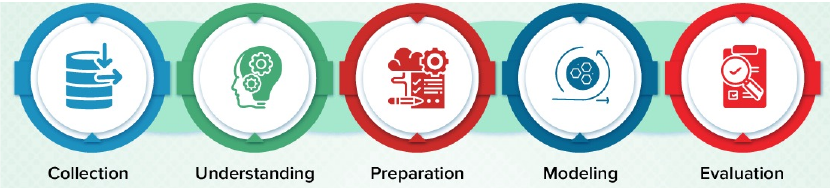
\includegraphics[width=.8\textwidth]{img/chapter-1/passi_CMCP.png}
    \centering
    \caption{Passi da effettuare per la CM e la CP}\label{img:passi}
\end{figure}

\subsection{Errori comuni nella System Evaluation}
Quando si fa systema evaluation, solitamente, si possono commettere degli errori, che possono portare poi ad avere uno scorretto parametro di confronto o giudizio del sistema. Gli errori che principalmente vengono fatti sono:
\begin{itemize}
  \item \textbf{Nessun obiettivo}: senza obiettivi chiari non esiste un modello universale; 
  gli obiettivi determinano tecniche, metriche e workload da usare, e non sono mai banali.
  
  \item \textbf{Obiettivi distorti}: porsi come obiettivo. Dimostrare che il nostro sistema è 
  migliore di un altro porta a una valutazione di parte, in cui gli analisti fanno da giudici invece che da osservatori imparziali.
  
  \item \textbf{Approccio non sistematico}: condurre la valutazione senza un metodo strutturato 
  (obiettivi $\rightarrow$ metriche $\rightarrow$ workload $\rightarrow$ esperimenti $\rightarrow$ analisi) 
  porta a risultati incompleti o non riproducibili.
  
  \item \textbf{Analisi senza capire il problema}: raccogliere dati e produrre grafici senza 
  aver compreso a fondo la natura del problema significa ottenere informazioni non utili alle decisioni.
  
  \item \textbf{Metriche di performance scorrette}: scegliere metriche che non riflettono gli 
  aspetti importanti del sistema (es. guardare solo il throughput quando è cruciale la latenza) porta a conclusioni fuorvianti.
  
  \item \textbf{Workload non rappresentativo}: utilizzare un carico artificiale che non riproduce 
  il comportamento reale degli utenti (picchi, mix di richieste, distribuzioni) rende i risultati poco affidabili.
  
  \item \textbf{Tecnica di valutazione sbagliata}: adottare un metodo inadeguato (analisi analitica, simulazione o misurazioni reali) 
  rispetto agli obiettivi porta a risultati poco significativi o addirittura falsati.
\end{itemize}

Dati tali errori di valutazione si comprende il motivo a cui è legato il bisogno di definire un path formale per la performance evaluation. Pertanto si va a definire una serie di passi sistematici che ci spiega come poter realizzare la syustem evaluation senza andare in contro alle problematiche descritte in precedenza. I passi da seguire sono i seguenti:
\begin{enumerate}
  \item Definire gli obiettivi e descrivere il sistema
  \item Elencare i servizi e i risultati attesi
  \item Selezionare le metriche
  \item Elencare i parametri
  \item Selezionare i fattori da studiare
  \item Scegliere la tecnica di valutazione
  \item Selezionare il workload
  \item Progettare gli esperimenti
  \item Analizzare e interpretare i dati
  \item Presentare i risultati
  \item Ripetere il processo
\end{enumerate}

Guardando tali passi si comprende che bisogna effettuare alcune scelte fondamentali. Le scelte che principalmente bisogna effettuare sono legate a: Tecniche di valutazione, Metriche di performance e Performance richieste

\subsubsection{Tecniche di valutazione}
Per valutare le performance di un sistema si possono utilizzare diverse tecniche che racchiudono una metodologia differente di approccio rispetto al sistema, che ci permette di poter valutare le prestazioni prescindendo dal sistema stesso (o in parte). Le tecniche principali di valutazione sono:
\begin{itemize}
    \item \textbf{Modellazione Analitica}: Si va a ricostruire il sistema mediante un modello matematico. Tale tecnica permette di avere una soluzione in forma chiusa (utilizza formule matematiche senza dover simulare o replicare un sistema). Tali sistemi, però, fanno delle assunzioni sul sistema, che permettono la semplificazione e la modellazione matematica
    
    \item \textbf{Simulazione}: Tale tecnica cerca di combinare la modellazione analitica del sistema con il mondo reale, cercando di emulare quanto più è possibile il caso reale tramite particolati software. \uppercase{è} una buona soluzione, poichè richiede un costo intermedio per essere effettuata; se non fosse per il tempo che bisogna dedicargli per la ricostruzione del sistema
    
    \item \textbf{Misura}: Si vanno a valutare le performance con misurazioni sul sistema reale. Tale approccio è il più costoso, sia in termini di carico che di costo, ma è il più efficiente poichè si è a contatto con il caso reale effettivo
\end{itemize}

Per selezionare la tecnica adatta al nostro caso bisogna fare una valutazione completa del sistema cercando quella che è la tecnica più adatta in base al nostro criterio di valutazione richiesto. Talvolta può essere anche possibile utilizzare più tecniche insieme. (Un esempio potrebbero essere i Twin Systems, dove vado ad effettuare modifiche prima in simulazione, e se noto miglioramento delle performance applico le stesse scelte anche al sistema reale andando ad analizzare ulteriormente le performance).

\subsubsection{Selezione della metrica}
Altro parametro importante da scegliere è la metrica da utilizzare. \uppercase{è} importante capire il corretto modo di scegliere una metrica dato che è il concetto su cui si basa il confronto tra vari sistemi. Le metriche possono basarsi su diversi criteri, i principali possono essere classificati come:
\begin{itemize}
    \item \textbf{Metriche per le performance}: Si vanno a valutare dei parametri di valutazione discreti (non probabilistici), dipendenti da: Tempo, Processing Rate, Consumo di risorse ecc.
    
    \item \textbf{Metriche per la Dependability}: Si va a valutare un sistema in base alla sua "efficenza", vista nel senso di probabilità di diversi eventi (guasti, eccezioni ecc.), esempi di tali metriche sono: Availability, Performability, Reliability ecc.
     
    \item \textbf{Metriche per i costi}: Si basano i criteri sui costi impiegati per l'implementazione di particolari sistemi
\end{itemize}

Uno dei criteri di selezione della metrica è quello presentato nell immagine [\ref{img:criterio-metrica}], che ci permette di capire, in base a come reagisci il sistema, quale tipologia e quale classe di parametri andare a considerare. Fare attenzione all'immagine, essa suddivide le possibili metriche in tre macroaree, la prima è quella riguardanti le metriche deterministiche, ovvero quelle metriche che vengono valutate su casi effettivi e risultati non di natura probabilistica; a differenza delle altre 2 categorie che, avendo a che fare con errori ecc., ricadono nei casi di dover andare a valutare il sistema mediante dei valori di natura probabilistica.

\begin{figure}
    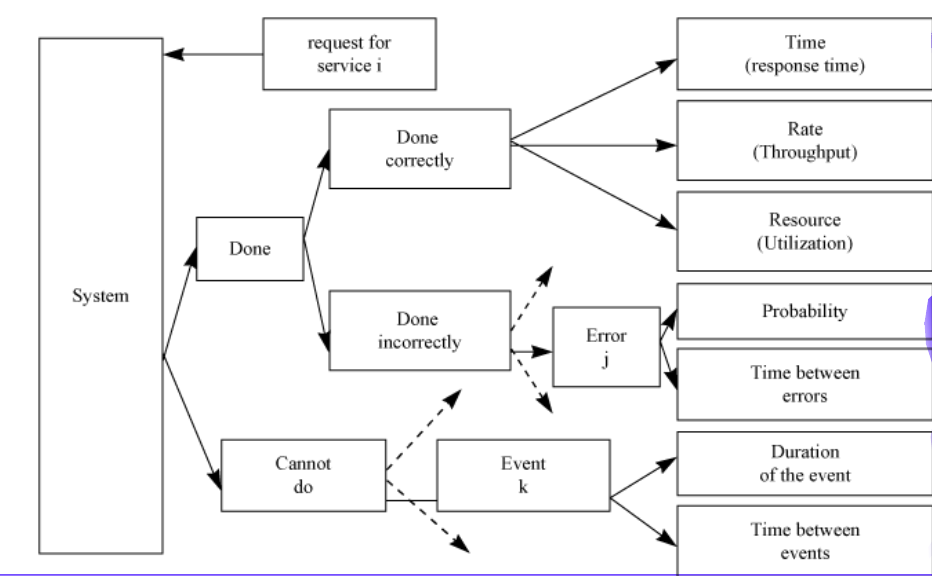
\includegraphics[width=.8\textwidth]{img/chapter-1/Metrics.png}
    \centering
    \caption{Criterio di selezione della metrica}\label{img:criterio-metrica}
\end{figure}

Le metriche presentate, quindi, sono le seguenti:
\begin{itemize}
    \item \textbf{Response Time}: Tale parametro ci permette di capire ogni quanto di tempo un sistema produce un risultato valido. Per la valutazione di tale parametro, però, possono essere effettuate varie tipologie di valutazione:
    \begin{itemize}
        \item \textbf{Response time}: Misurazione basata sul tempo tra l'inizio e la fine della richiesta
            
        \item \textbf{Reaction time:} Fine della richiesta dall'inizio del suo processamento
        
        \item \textbf{Turnaround time:} Inizio della richiesta fino alla fine della risposta
    \end{itemize}

    Generalmente la Response Time cresce all'aumentare del carico sul sistema, per tale caso è stato definito quello che verrà chiamato \textbf{Strech Factor} (permette di capire quando non saranno più usabili un certo numero di risorse)

    \item \textbf{Processing Rate}: Il processing rate non rappresenta altro che il throughput associato al mio sistema, e che quindi calcola la quantità di lavoro svolto da un singolo componente per unitò di tempo.
\end{itemize}

Talvolta, utilizzare sia il thoroughput che il response time può risultare ridondante, pertanto si decide di utilizzare un unico parametro, dipendente da entrambi, chiamato \textbf{potenza}, che si può calcolare come \textbf{\(\frac{Throughput}{Response Time}\)}. Pertanto è giusto andare a ridefinire anche i diversi punti di evoluzione della potenza, che racciudono la nostra attenzione

\begin{itemize}
    \item \textbf{Capacità nominale:} Rappresenta il throughput massimo raggiungibile in condizioni di carico di lavoro ideali. Tuttavia, a questo livello di throughput, il tempo di risposta è generalmente troppo elevato.
    \item \textbf{Capacità utilizzabile:} È il throughput massimo che si può ottenere, quindi è il punto massimo dopo il quale il sistema potrebbe andare in crash (quindi ad esempio ha tempi di risposta molto lunghi ma riesce a gestire molto più carico)
    \item \textbf{Capacità di "ginocchio":} È il punto operativo ottimale, considerato il miglior equilibrio tra un alto throughput e un basso tempo di risposta. Questo punto corrisponde al valore massimo della metrica Power.
\end{itemize}

Oltre la potenza un ulteriore parametro utile è la \textbf{fairness}, che ci permette di capire se un aprticolare sistema distribuisce bene il carico o meno. Ciò lo veniamo a scoprire mediante il calcolo del preciso valore di fairness che è normalizzato, e quindi compreso tra 0 ed 1.

A livello formale, si definisce:

\begin{itemize}
    \item \(x_i\), frazione del throughput associato ad \(x_i\)
    \item n, numero di utenti nel sistema
\end{itemize}

A questo punto comprendo se sto usando il throughput in maniera fair, calcolando la \textbf{fairness}, che mi dice che se ogni utente ha a disposizione una porzione eguale di throughput, allora sarà 1, mentre nel caso opposto sarà vicino allo 0.
Per calcolare la fairness si utilizza la seguente formula:

\Large
\[
fairness = \frac{\left(\sum_{i=1}^{n}x_i\right)^2}{n\sum_{i=1}^{n}x_i^2}
\]
\\\\
\normalsize

Con tale formula si comprende che se tutti i throughput \(x_i\) sono uguali allora => \(fairness = 1\).


\chapter{Workload}
Un Workload, nella sua definizione di base, è: \textit{Tutti i possibili input che un sistema riceve in un certo periodo di tempo}
\\
Tale definizione, pertanto, prescinde dalla sola valutazione delle performance. Nel caso specifico i workload che sono utilizzati nella valutazione delle performance sono detti \textbf{test workload}, tali test workload possono essere generati e categorizzati secondo particolari tecniche di utilizzo e schematizzazione

\section{Test Workload}
I test Workload sono dei normali workload utilizzati per gli studi delle performance. In generale, i test workload possono essere classificati in due particolari categorie:
\begin{itemize}
    \item \textbf{Workload Reali}: Workload che sono caratterizzati dall'osservazione di specifici casi reali
    \item \textbf{Workload Sintetici}: Workload che sono caratterizzati da pochi parametri ma che cercano di replicare quelli che potrebbero essere dei workload reali
\end{itemize}

Le due classificazioni differiscono fortemente sotto molti punti di vista. Il principale tipo di workload utilizzato è quello sintetico, dato che viene caratterizzato tramite pochi parametri e può essere replicato senza dover tenere memoria di un workload reale (che richiederebbe memorie molto ingenti per essere memorizzato).

\subsection{Addition Istruction}
L'\textbf{Addition Istruction} è una tecnica di workload sintetico per i computer systems. Essa è stata utilizzata in passato per la valutazione delle performance sui vari computer e comprendeva quello di valutare la velocità e l'efficienza dell'operazione di addizione (Operazione più usata all'interno dei programmi passati).

\subsection{Instruction Mixes}
L'\textbf{Istruction Mixes} è un evoluzione dell'Addition Istruction, poichè non va a considerare solo l'operazione di addizione intera, ma anche tutte le altre istruzioni possibili. Per avere uno schema più adatto alla sintetizzazione di un workload si hanno delle specifiche di Istruction Mixes, che non sono altro che tabelle che listano le varie \textbf{classi di istruzioni} con la loro "percentuale" di utilizzo (frequenza). In questo modo sarà possibile, andare a selezionare a caso le istruzioni, rispettando la distribuzione descritta dall'Istruction Mixes.

\subsubsection{Disadvantages}
La complessità sempre crescente delle architetture e quindi delle classi di istruzioni, non viene riflessa all'interno delle tabelle di istruction mixes, pertento risulta difficile valutare completamente la totalità dell'architettura. Oltre alla complessità delle classi, incidono anche i tempi di esecuzione, che è altamente variabile e dipendente da diversi parametri quali:
\begin{itemize}
    \item \textbf{Modalità di indirizzamento}: Come le modalità di indirizzamento diretto o indiretto di un architettura
    \item \textbf{Cache Hit}: Probabilità di trovare il dato su cui si vuole lavorare in Cache
    \item \textbf{Pipeline Efficiency}: Se la pipeline mantiene per molto tempo l'esecuzione di un comando per ciclo di clock (ad esempio gestendo bene la questione dei salti e della branch prediction)
    \item \textbf{Interferenza dei dispositivi esterni durante i cicli di accesso processore-memoria}: Ad esempio concorrenza dei bus mentre si accede alla memoria per il prelievo di un dato
\end{itemize}

Oltre a problematiche di tipo puramente architetturale e strutturale, il tempo di esecuzione può variare anche in base alla forma e alle operazioni che devono essere fatte sui dati, come operazioni del tipo:
\begin{itemize}
    \item La frequenza con cui compare lo zero come parametro
    \item Quante volte compare lo zero in operazioni di moltiplicazione
    \item il numero medio di spostamenti richiesti in un'operazione in virgola mobile
    \item numero di volte in cui un ramo condizionale viene eseguito 
\end{itemize}

Oltretutto, le combinazioni di istruzioni delle istruction mixes non riflettono le funzionalità di indirizzamento virtuale della memoria

\subsubsection{Considerazioni}
Nonostante le varie problematiche che porta con se, l'istruction mixes, ci permette comunque di poter avere un singolo parametro di confronto tra sistemi diversi. Il parametro è un numero che esprime l'inverso del tempo di esecuzione e può essere espresso come:
\begin{itemize}
    \item \textbf{MIPS (Millioni di Istruzioni Per Secondo)}
    \item \textbf{MFLOPS (Millioni di FlOaring Point istructionS)}
\end{itemize}

Però un'altro problema legato a questo valore è che stima le prestazioni solo del \textbf{processore} e quindi \textbf{non dell'intero sistema}. Il divario tra le performance reali e non dei sistemi che vengono valutati con tali modelli è fatto, quindi, solo dalla differenza dei programmi che vengono eseguiti, e quindi non è una statistica affidabile per una tipologia generale di applicazioni.

\subsection{Kernels}
I \textbf{Kernels} sono un'evoluzione dell'istruction mixes, poichè non vanno a considerare più le istruzioni nella loro singolarità, ma vanno a considerare dei gruppi di istruzioni (delle funzioni). Le funzioni, in particolare, sono dette \textbf{kernel} e sono implementare solo per il consumo della CPU, quindi nessuna prevede o fa uso dei dispositivi di I/O (almeno nelle loro versioni iniziali, dato che oggi tale classe di kernel è chiamata processing kernel). Il nome \textbf{kernel} viene dal fatto che si vuole identificare una serie di passaggi chiave che poi sono utilizzati nelle più comuni applicazioni. Ad esempio si possono utilizzare tutti i passaggi che servono per il calcolo dell'inverso di una matrice o di tutte le operazioni che vengono richieste da un algoritmo di sorting. Difatti le tecniche più utilizzare ad oggi che rispettano un modello kernel sono:
\begin{itemize}
    \item \textbf{Sieve}: Algoritmo per trovare tutti i numeri primi fino ad N (\href{https://it.wikipedia.org/wiki/Crivello_di_Eratostene}{Crivello di Eratostene})
    \item \textbf{Puzzle}: Algoritmi per la risoluzione del gioco del 15, le N-Regine o il Sudoku
    \item \textbf{Tree Searching}: Operazioni che possono essere effettuate all'interno di un'albero
    \item \textbf{Ackermann's Function}: Funzione matematica e molto ricorsiva che permette di valutare la reazione e la gestione di tali chiamate (\href{https://it.wikipedia.org/wiki/Funzione_di_Ackermann}{funzione di Ackermann})
    \item \textbf{Matrix Invertion}: Va a valutare il comportamento del sistema rispetto alle operazioni che bisogna effettuare per ottenere l'inverso di una matrice NxN (anche tramite diversi metodi di calcolo)
    \item \textbf{Sorting}: Agglomerato di algoritmi di ordinamento differenti
\end{itemize}

Però, molti dei problemi che ritroviamo all'interno dell'istruction mixes si ripercuotono anche sull'utilizzo dei kernels, quali tutti i problemi dipendenti dall'applicazione e dalla forma dei dati e non instrinsecamente dall'architettura (dove vi è sempre la mancanza però della gestione dei dispositivi di I/O)

\subsection{Application Benchmarks}
Gli \textbf{Application Benchmarks} sono dei workload che vengono costruiti in base all'applicazione che si sta andando a testare. Quindi si vanno a verificare i casi d'uso di un'applicazione in base all'impiego che ne devo fare. Nella letteratura, in realtà, benchmark viene utilizzato come sinonimo di workload, pertanto molte volte le tecniche come quella dei kernel (test di funzioni e non di singole istruzioni), vengono visti come benchmark. Il processo che vuole valutare le performance in base ad un determinato benchmark viene detto \textbf{benchmarking}. L'application benchmark, quindi, fa riferimento e cerca di replicare un workload reale in base alla tipologia di applicazione che voglio andare a valutare, ad esempio, se voglio valutare un servizio bancario è inutile che vada a testare delle funzioni di high performance sul processore (dato che non vengono mai fatte), ma vada a valutare la qualità di utilizzo e di controllo del database. 

In generale, per confrontare due sistemi, posso utilizzare i benchmark, oltretutto, una cosa importante di caratterizzazione dei benchmark, sono le proprietà che essi devono mantenere, ovvero:
\begin{itemize}
    \item \textbf{Representativeness}(Rappresentatività): Si garantisce che il benchmark sia rappresentativo di un workload reale che si vuole andare a valutare 
    \item \textbf{Portability}: Il benchmark deve poter essere eseguito su piattaforme diverse, e quindi non dipende dalla macchina e dall'hardware di un sistema specifico
    \item \textbf{Repeatability}: Eseguendo più volte lo stesso benchmark nelle stesse condizioni, i risultati devono essere coerenti. Questo garantisce l’affidabilità e la robustezza delle misure
    \item \textbf{Scalability}: Il benchmark deve poter funzionare su sistemi di dimensioni diverse (ad esempio da un singolo nodo a un cluster) e adattarsi a diversi livelli di carico, senza perdere significato
    \item \textbf{Non-intrusiveness}: L’esecuzione del benchmark non deve alterare significativamente il comportamento del sistema misurato. Deve misurare senza influenzare in modo rilevante le prestazioni stesse
    \item \textbf{Easy-to-use}: Deve essere semplice da configurare, avviare ed eseguire, in modo che chiunque possa utilizzarlo senza particolari complessità tecniche
    \item \textbf{Easy-to-understand}: I risultati prodotti devono essere chiari e facilmente interpretabili, anche da chi non è un esperto tecnico
\end{itemize}

La cosa importante quando si sceglie un benchmark e trovare uno specifico \textbf{agreement}, e quindi un accordo su quale tipologia di applicazione andare a testare. In generale un benchmark nasce per poter comparare diverse tipologie di strutture, di componenti e di architetture, rispettando però lo specifico agreement, che oltre a dare un ordine a quello che si vuole testare, permette di comparare le diverse architatture per lo specifico compito che andranno a svolgere (sempre in linea con l'agreement).

\subsection{Esempi di benchmark}
\subsubsection{Sieve}
Algoritmo che utilizza il criterio di Eratostene per la determinazione dei numeri primi da 0 ad N, con N dato in ingresso all'algoritmo. Il suo funzionamento principale è quello di partire da tutti i numeri interi da 1 ad N, e poi eliminare tutti i multipli dei valori (in ordine), da 1 a \(\sqrt{N}\). I valori che però vengono considerati sono solo quelli non eliminati.
Per esempio:
\\
N = 20, \(\sqrt{20} \approx 5\)
\[
\text{Passo 0: }[\underline{1},\underline{2},\underline{3},\underline{4},\underline{5},\underline{6},\underline{7},\underline{8},\underline{9},\underline{10},\underline{11},\underline{12},\underline{13},\underline{14},\underline{15},\underline{16},\underline{17},\underline{18},\underline{19},\underline{20}]
\]
\[
\text{Passo 1: }[1,\underline{2},\underline{3},\underline{4},\underline{5},\underline{6},\underline{7},\underline{8},\underline{9},\underline{10},\underline{11},\underline{12},\underline{13},\underline{14},\underline{15},\underline{16},\underline{17},\underline{18},\underline{19},\underline{20}]
\]
\[
\text{Passo 2 (eliminazione multipli di 2): }[1,\underline{2},\underline{3},4,\underline{5},6,\underline{7},8,\underline{9},10,\underline{11},12,\underline{13},14,\underline{15},16,\underline{17},18,\underline{19},20]
\]
\[
\text{Passo 3 (eliminazione multipli di 3): }[1,\underline{2},\underline{3},4,\underline{5},6,\underline{7},8,9,10,\underline{11},12,\underline{13},14,15,16,\underline{17},18,\underline{19},20]
\]
\[
\text{Risultato finale: }[1,\underline{2},\underline{3},4,\underline{5},6,\underline{7},8,9,,10,\underline{11},12,\underline{13},14,15,16,\underline{17},18,\underline{19},20]
\]

\subsubsection{Algoritmo di Ackermann}
Tale algoritmo è adatto per lo studio delle chiamate ricorsive, dato che costituisce la funzione ricorsiva più pura. In generale con tale tipologia di struttura si può andare a valutare bene:
\begin{itemize}
    \item \textbf{Tempo di esecuzione medio per le call}
    \item \textbf{Numero di istruzioni eseguite per call}
    \item \textbf{Stack space per le call}
\end{itemize}

\subsubsection{SPEC Benchmark Suite}
Corporazione non profit che ha stilato una serie di bechmark (circa una decina), che possono essere utilizzati per valutazioni di varia natura. Essi sono una base per la valutazione più generale dei sistemi a prescindere dalla loro struttura architetturale


\chapter{Tecniche di caratterizzazione dei workload}
I workload reali sono la migliore opzione per andare a valutare le performance specifiche di un dato sistema, il problema è che mantenere tale workload richiede un ingente quantità di memoria. Quindi è nata la necessità di trovare e ricercare delle tecniche che permettessero di poter caratterizzare un workload reale e ridurre la quantità di dati da memorizzare per poterne avere una statistica quanto meno affidabile

\section{Terminologia}
Gli argomenti che saranno affrontati durante tale capitolo richiedono una conoscenza della specifica terminologia utilizzata. In generale i concetti fondamentali da conoscere inerenti al dispositivo ed al componente da testare sono:
\begin{itemize}
    \item \textbf{DUT}(Device Under Test): Sistema che viene sottoposto ad uno specifico test (es. CPU o un processo di transazione)
    \item \textbf{CUT}(Component Under Test): Componente del sistema di cui si vogliono conoscere le performance (es.ALU o Unità Disco)
    \item \textbf{Metrica}: Metrica che si vuole andare a valutare per il CUT (es. MIPS o T/s)
\end{itemize}

\begin{figure}[h]
\centering
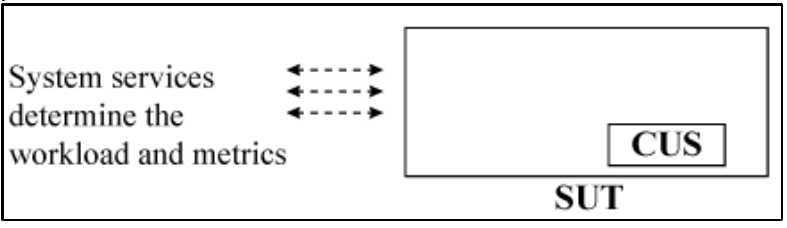
\includegraphics[width=.8\textwidth]{img/chapter-3/CUS-SUT.png}
\caption{Struttura del sistema di test}\label{img:cus-sut}
\end{figure}

Oltre la terminologia intrinseca al sistema di test bisogna definire anche la terminologia inerente ad altre entità interagenti. Quindi si definiscono i seguenti termini:
\begin{itemize}
    \item \textbf{User}: entità che esegue le richieste di servizio
    \item \textbf{Workload components}(Qualitative identifiers): Componenti basilari che mi permettono di capire a livello qualitativo cosa fa un workload, quindi la natura e la struttura delle attività che vengono svolte dalle varie componenti (es. transazione in un database, una query in un motore di ricerca o Un processo o thread in un sistema operativo)
    \item \textbf{Workload parameters}(Quantitative Identifiers): Sono parametri quantitativi associati al workload e che quindi descrivono come le componenti si comportano. Servono principalmente per avere una misura numerica delle caratteristiche del workload (es. Arrival rate [Quante richieste al secondo], il service time [quanto tempo serve per completare un compito], Resource Usage [quante risorse vengono consumate], I/O operations [quante lettura/scritture su disco avvengono])
\end{itemize}

\section{Workload Characterization Tecniques}
\begin{info}
La \textbf{Workload Characterization} è un processo che permette di definire un workload di test di dimensione ridotta, ma che conservi tutte le caratteristiche e le proprietà (sia statiche che dinamiche), del workload reale. Ciò ne permette la replicazione e l'utilizzo in ambito di performance analysis.
\end{info}
C'è però da capire come sia possibile estrarre il workload sintetico dal workload reale, pertanto sono state utilizzare e definite diverse tecniche negli anni. L'obbiettivo principale di tali tecniche è quello di trovare dei parametri ridotti con cui cercare di poter descrivere il workload reale a meno di una certa quantità di informazione persa (tale quantità saraà valutata in vari modi, solitamente si utilizzerà la varianza o la devianza).

\subsection{Averaging}
La tecnica dell'\textbf{Averaging} è molto semplice, cerca di ridurre il workload in una singola istanza i cui parametri vengono valutati con la media dei parametri presenti nel workload reale. Quindi quello che si va a fare è:
\\
Siano: \({x_1,x_2, \dots, x_n}\) i valori assunti nel workload dal parametro \(x\), allora si può approssimare tale parametro tramite la media aritmetica definita come:
\[
\overline{x} = \frac{1}{n}\sum_{i=1}^{n}x_i
\]
Talvolta però non è proprio l'ideale utilizzare la media, ciò dipende fortemente dalla tipologia di dati che si ha. Solitamente si potrebbe pensare di utilizzare altre tecniche come: la mediana (permette di prendere un valore appartenente al workload più centrale), oppure il 50-percentile, la media geometrica ecc.

\subsubsection{Specifying Dispersion}
Caratterizzare un workload reale mediante un workload sintetico prevede di avere, intrinsecamente, degli errori. Ciò accade principalmente per la limitatezza che ho nei parametri che voglio andare a considerare (non posso avere memoria di tutte le istanze del workload reale, ma solo di alcune di esse).
Si potrebbe pensare di andare a stimare l'errore mediante la somma di tutte le deviazioni, ovvero:
\[
errore\_totale = \sum_{i=1}^{n}(x_i-\overline{x})
\]
Tale rappresentazione, però, non è proprio utile, il problema principale risiede nel segno che possono avere le deviazioni (immaginiamo il caso di avere 5 e 15, la media è 10, ma l'errore, se calcolato con la formula sopra è 0 [(5-10) + (15-10)]), il che porta a rendere tale ragionamento errato.
Un'altra soluzione potrebbe essere quella di andare a considerare la deianza, ovvero la somma degli errori quadratici
\[
errore\_totale = \sum_{i=1}^{n}(x_1 - \overline{x})^2
\]

La devianza, quindi, risolve il problema del segno delle deviazioni, ma dipende fortemente dal numero di dati.
Data quindi tale dipendenza dal numero di dati della devianza, si preferisce utilizzare la \textbf{varianza campionaria}, che va a dividere la devianza per n - 1. Si va a considerare n - 1 per  via dei gradi di libertà, ovvero, il numero di deviazioni linearmente indipendenti [warning successivo]
\[
s^2 = \frac{1}{n-1}\sum_{i=1}^{n}(x_i-\overline{x})^2
\]

\begin{warn}

\textit{Tale dimostrazione non è stata fatta in aula, per quanto sia semplice non è richiesta ai fini dell'esame ma solo per questione di conoscenza personale.}\\ 
Tale formula ci fa capire perchè dividiamo per n-1 nella varianza capionaria e perchè tale divisione è giustificata come il numero di \textbf{gradi di libertà}
\[
\sum_{i=1}^{n}(x_i - \overline{x}) = \sum_{i=1}^{n}x_i - \sum_{i=1}^{n}\overline{x} = \sum_{i=1}^{n}x_i - \overline{x} \sum_{i=1}^{n}1 = \sum_{i=1}^{n}x_i - n \overline{x} = 
\]
\[
=\sum_{i=1}^{n}x_i - n \left(\frac{1}{n}\sum_{i=1}^{n}x_i\right) =\sum_{x=1}^{n}x_i - \sum_{x=1}^{n}x_i = 0
\]

Dopo tale dimostrazione si comprende che le devianze linearmente indipendenti sono n-1, dato che una sarà esprimibile come somma delle altre
\end{warn}

Oltre al concetto di varianza, solitamente, si preferisce parlare di deviazione standard, dato che è espressa nell'unità di misura della grandezza che si sta andando a valutare. La deviazione standard si calcola come radice quadrata della varianza campionaria, ovvero:
\[
s = \sqrt{s^2}
\]

Oltre a tale valore, per rendersi conto dell'incertezza rispetto ai dati effettivi (essere in grado di confrontare un sistema piccolo con un sistema grande cercando di evitare un confronto rispetto alle grandezze di misura), è utile considerare il \textbf{coefficente di variazione}, che viene definito come:
\[
COV = \frac{s}{\overline{x}}
\]

Un esempio di utilizzo di tale valore è il seguente:
Immaginiamo di avere due sistemi e di averne valutato il tempo di risposta e la deviazione standard associata ad ogni sistema. Si avrà il seguente scenario:
\begin{itemize}
    \item \textbf{Sistema 1}: response time = 10 ms, dev. standard = 2 ms
    \item \textbf{Sistema 2}: response time = 200 ms, dev. standard = 15 ms
\end{itemize}

Se mi chiedessi quale dei due sistemi risulta più \textbf{stabile}, allora intuitivamente andrei a confrontare le dev. standard e valuterei quella minore come più stabile. Ma questo, però, non viene messo a confronto con gli andamenti medi (non guardo la larghezza della campana rispetto alla sua altezza [gaussiana]). Pertanto se calcolo i coefficenti di variazione, avrò che per il sistema 1: COV = 0,2 = 20\%; mentre per il sistema 2: COV = 0,075 = 7,5\%. Il che mi dimostra che il sistema 2 è più stabile rispetto al sistema 1 (completamente il contrario rispetto alla decisione iniziale).

\subsection{Single Parameter Histogram}
Il \textbf{Single Parameter Histogram} si occupa di costruire un istogramma delle occorrenze che vada a caratterizzare il \textbf{singolo parametro} considerato ed analizzato. La costruzione di un istogramma viene effettuata andando a valutare la frequenza di occorrenza di un dato valore in base ad una sua distribuzione discreta. 

Più formalmente quello che si va a costruire è una funzione \(f(x)\) che mi dice quante volte il parametro \(x\) assume un certo valore. Tale funzione viene costruita andando a suddividere l'intervallo di valori che il parametro può assumere in \textbf{buckets} (o bins), ovvero sottointervalli. Quindi si va a contare quante volte il parametro assume un valore compreso in un certo bucket e si va a riportare tale conteggio sull'asse delle ordinate, mentre sull'asse delle ascisse si riporta il bucket considerato.

Vi sono però dei problemi nell'utilizzare tale tecnica, utilizzare un istogramma per ogni parametro vuol dire utilizzare grandi quantità di memoria, a livello numerico:
Consideriamo \(n \)bucket  per ogni valore (intervalli di cui si deve tenere traccia), \(m\) il numero di parametri per ogni componente, ed \(k\) il numero di componenti, allora la memoria richiesta per memorizzare tale istogramma sarà:
\[
Memoria = n m k
\]

Ciò risulta troppo dettagliato per la reppresentazione del workload, oltretutto, tale metodo non tiene conto delle correlazioni tra i vari parametri, dato che ogni istogramma viene costruito in maniera indipendente dagli altri, ciò porta quindi a portare all'interno della descrizione del workload anche parametri che potrebbero essere deducibili da altri (ridondanza di informazioni). Questo pregiuduca anche la possibilità di selezionare i parametri da considerare mediante la varianza, dato che dati che non sono indipendenti porterebbero la stessa quantità di informazione.

\subsection{Multiparameter Histogram}
Il \textbf{Multiparameter Histogram} è una tecnica che cerca di risolvere i problemi del single parameter histogram, andando a considerare le correlazioni tra i vari parametri. Quello che si va a fare è costruire un istogramma che consideri non swolo le frequenze di un singolo parametro, ma le frequenze di n-parametri, correlate tra di loro. Per comprendere la complessità nella costruzione di un istogramma a n-variabili, vediamo un esempio con due variabili, che sarebbe quello mostrato in figura [\ref{img:multi-histograms}]. Per leggere tale grafico dobbiamo considerare 3 assi, che nel nostro caso sono rappresentati come:
\begin{itemize}
    \item \textbf{Asse X}: rappresenta il range di valori del primo parametro
    \item \textbf{Asse Y}: rappresenta il range di valori del secondo parametro
    \item \textbf{Asse Z}: Viene rappresentato mediante la griglia quadrettata, ed il valore considerato è il numero di punti che sono presenti per un dato intreccio di valori.
\end{itemize}

Ciò ci aiuta a capire come si possono trovare dei pattern tra i vari parametri, data la specifica distribuzione dei parametri (in questo caso le due variabili crescono l'una rispetto all'altra). La problematica principale risiede nella quantità di parametri che bisognerebbe incatenare per trovare delle correlazioni tra le variabili, ed oltretutto, per workload molto grandi risulta complicato andare a memorizzare tale quantità di dati anche andando a considerare un filtro con la varianza.

\begin{figure}[h]
\centering

\begin{subfigure}[b]{0.8\textwidth}
\centering
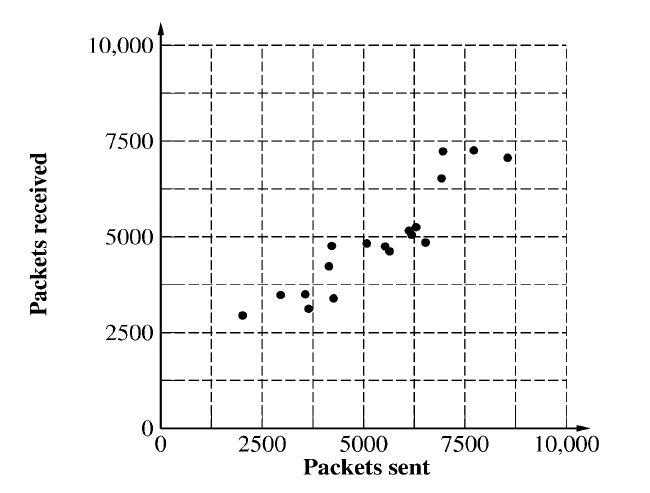
\includegraphics[width=\textwidth]{img/chapter-3/multi-histogram.png}
\caption{Multiparameter Histogram on 2D space}\label{img:multi-histogram}
\end{subfigure}

\hfill

\begin{subfigure}[b]{0.8\textwidth}
\centering
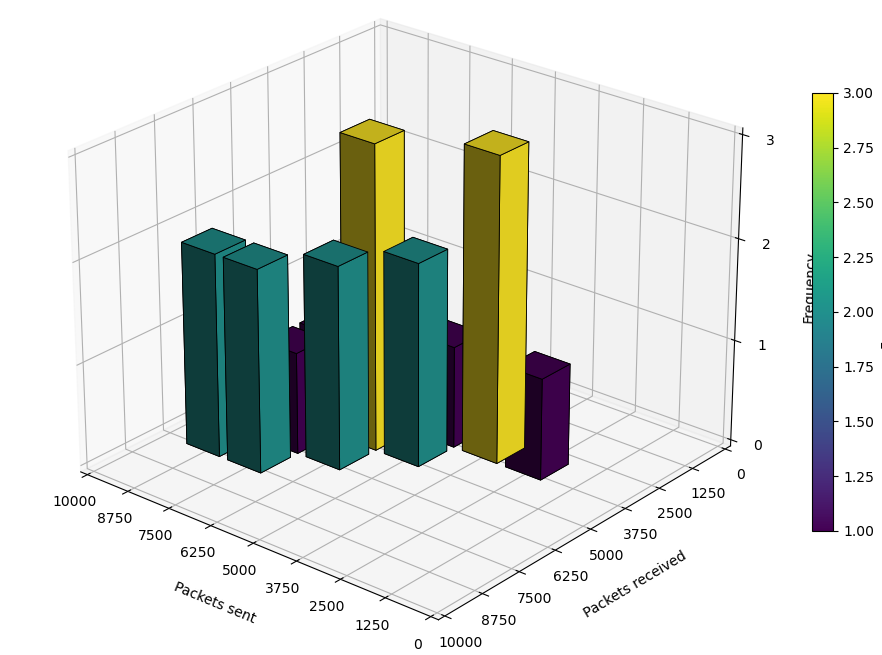
\includegraphics[width=.8\textwidth]{img/chapter-3/multi-histogram-3d.png}
\caption{Multiparameter Histogram on 3D space}
\label{img:multi-histogram-3d}
\end{subfigure}

\caption{Esempi di istogrammi multiparametrici}\label{fig:multi-histograms}
\end{figure}

\clearpage
\subsection{Principal Component Analysis (PCA)}
Un modo utilizzato per ridurre il numero di parametri con cui andare a rappresentare le istanze del workload è la \textbf{Principal Component Analysis (PCA)}. Tale tecnica ha come compito quello di trasformare l'insieme di istanze in altre istanze, le nuove istanze vengono definite sulla base delle componenti principali (che differiscono dai parametri reali), poichè nel nuovo spazio, tali parametri sono tutti linearmente indipendenti, e non ci sono correlazioni. Il funzionamento matematico della PCA è basato sull'effettuazione di una media pesata per ogni parametro. Precisamente:
\\
Dati i parametri \({x_1,x_2,\dots,x_N}\), si vuole trovare un nuovo insieme di parametri \({y_1,y_2,\dots,y_N}\), voglio però che l'insieme di parametri \(y_i\) sia linearmente indipendente, e che la varianza di ogni parametro \(y_i\) sia massimizzata. Di base per vedere come andare a costruire la matrice di trasformazione della PCA, si dovrebbe calcolare la matrice di covarianza, una volta calcolata si valutano gli autovettori di tale matrice, che costruiranno poi la matrice di trasformazione finale. Gli autovettori, quindi, rappresentano le direzioni principali e sono disposti in maniera che la prima componente principale sia quella con la varianza maggiore. Difatto si sta andando a fare una media pesata dei parametri per costruire il valore della nuova componente principale. Precisamente:
\[
y_j = \sum_{i=1}^{N}w_{ij}x_{ij}
\]

Tale formula va letta in questo modo:
\begin{itemize}
    \item \textbf{\(y_j\)}: rappresenta la j-esima componente principale
    \item \textbf{\(x_{ij}\)}: rappresenta il valore del parametro \(i\) nell'istanza \(j\)
    \item \textbf{\(w_{ij}\)}: rappresenta il peso associato al parametro \(i\) per la j-esima istanza
\end{itemize}

Per effettuare la PCA bisogna seguire i seguenti passi:
\begin{enumerate}
    \item Andare a calcolare la matrice di covarianza dei dati (prima si potrebbero effettuare anche operazioni di normalizzazione)
    \item Andare a calcolare gli autovettori e gli autovalori della matrice di covarianza
    \item Costruire la matrice di trasformazione mediante gli autovettori ordinati secondo gli autovalori in maniera decrescente (gli autovalori portano con loro la quantità di varianza, quindi ordinando gli autovettori si avrà uno spazio in cui il primo parametro copre la maggior varianza [utile per la selezione di un minor numero di parametri])
\end{enumerate}

In maniera più compatta, quindi, effettuata la PCA, si avrà che:
\begin{itemize}
    \item I nuovi parametri y sono calcolabili come combinazioni lineari dei parametri x
    \item I parametri y sono linearmente indipendenti, dato che il prodotto interno tra due parametri y è 0
    \item Il nuovo set di parametri y è ordinato in maniera tale che la varianza del primo parametro è maggiore della varianza del secondo e così via
\end{itemize}

\subsubsection{Z-Score Normalization}
La \textbf{z-score normalization} è una tecnica che permette di andare a normalizzare i dati, in maniera tale che ogni parametro abbia media 0 e deviazione standard 1. Tale tecnica è utile per poter effettuare la PCA, dato che si vuole evitare che parametri con range di valori molto diversi tra di loro possano influenzare in maniera sproporzionata il risultato finale. La formula per effettuare tale normalizzazione è la seguente:
\[
x'_s = \frac{x_{s} - \overline{x_s}}{s_{x_s}}
\]

Tale operazione permette di poter confrontare i parametri con un distribuzione normale, il che, quindi, andrà a rappresentare i dati come distanza da 0 e rappresentato secondo la deviazione standard s. Ciò ci permette anche di poter confrontare i dati tra di loro, senza andarea a considerare il range di valori che possono assumere.

\subsection{Clustering}
Mediante l'utilizzo della PCA si è andata ad effettuare la riduzione della quantità di parametri rappresentativi di un istanza (o componente) del workload. Per ridurre ancora di più la quantità di dati di rappresentazione del workload, si può andare ad effettuare una riduzione della quantità di istanze stesse. Per effettuare tale riduzione si fa utilizzo del \textbf{Clustering}, che è una tecnica di apprendimento non supervisionato che permette di andare a raggruppare le istanze in base alla loro similarità. Ciò richiede anche che la rappresentazione delle istanze sia adeguata per trovare degli specifici agglomerati di dati. (Per comprendere meglio, guardare la figura [\ref{img:clustering}], se i dati non fossero ben divisi non potrei creare i cluster per bene dato che avrei molta confusione). Una volta raggruppate le istanze, si può andare a rappresentare ogni cluster mediante un'unica istanza rappresentativa (solitamente la media dei parametri delle istanze che compongono il cluster). In questo modo si va a ridurre la quantità di istanze da memorizzare, andando a perdere però una certa quantità di informazione (che può essere valutata mediante la varianza o la devianza).

\begin{figure}[h]
\centering
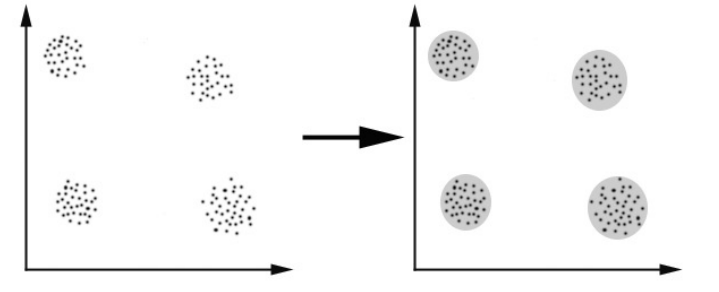
\includegraphics[width=.6\textwidth]{img/chapter-3/Clustering.png}
\caption{Esempio di clustering}\label{img:clustering}
\end{figure}

Per effettuare il clustering, generalmente, si eseguono i seguenti passaggi:
\begin{enumerate}
    \item Prendere un insieme di istanze appartenenti al workload (o ad una sua trasformazione mediante PCA)
    \item Scegliere i parametri del workload da considerare per effettuare la clusterizzazione (omettere i parametri che portano una quantità di varianza bassa)
    \item Selezionare una metrica di distanza (utile per la valutazione della similarità tra le istanze)
    \item Trattazione degli outliers (dati che sono molto distanti dagli altri, e che potrebbero falsare il risultato finale)
    \item Data scaling (utile per evitare che parametri con range di valori molto diversi tra di loro possano influenzare in maniera sproporzionata il risultato finale)
    \item Effettuare il clustering (utilizzando uno degli algoritmi di clustering esistenti)
    \item Interpretazione dei risultati (andare a valutare la qualità del clustering effettuato)
    \item Cambiare i parametri e/o il numero di cluster e ripetere i passi dal 3 al 7
    \item Selezionare un componente rappresentativo per ogni cluster
\end{enumerate}

\begin{warn}
Negli appunti si fa utilizzo del termine \textbf{istanza}, che per il seguente ambito è sinonimo di \textbf{componente}. Tale termine viene utilizzato per indicare un'entità del workload che viene caratterizzata da un insieme di parametri.
\end{warn}

\subsubsection{Campionamento delle componenti}
Il \textbf{Campionamento delle istanze} è una tecnica che va a selezionare un sottoinsieme di componenti del workload prima di proseguire nell'algoritmo di clustering. Ciò è dovuto al fatto che gli algoritmi di clustering sono computazionalmente costosi, e pertanto si cerca di ridurre la quantità di dati da considerare. La tecnica di selezione delle componenti da andare a considerare può essere di varia natura. Precisamente si studiano (per il seguente corso), le seguenti tecniche:
\begin{itemize}
    \item \textbf{Random Sampling}: Si va a selezionare un sottoinsieme di componenti in maniera casuale
    \item \textbf{Resource Consuption Based Sampling}: Si va a selezionare un sottoinsieme di componenti in base alla quantità di risorse che esse consumano (si vanno a selezionare le componenti che consumano più risorse)
\end{itemize}

Per capire se ho effettuato un buon campionamento, una volta effettuato il clustering vado a vedere, sul workload intero, se posso associare le componenti mancanti ai cluster trovati. Se il numero di componenti non assignabili è alto allora è indice di un cattivo campionamento.

\subsubsection{Selezione dei parametri}
Vado a selezionare un sottoinsieme di parametri rtappresentativi delle componenti. Tali parametri devono essere scelti in maniera tale che siano in grado di rappresentare la maggior quantità di varianza possibile o rispetto all'impatto sulle performance. Per fare ciò si può utilizzare la PCA, andando a selezionare i parametri che portano più varianza. Facendo in questo modo introduco una quantità di varianza persa a discapito, però, della riduzione della dimensionalità del problema, e di conseguenza, della riduzione del tempo speso per effettuare la clusterizzazione.

\subsubsection{Metrica di distanza}
Una metrica di distanza mi permette di calcolare la ditanza tra varie componenti in spazi n-dimensionali, dove n è il numero di parametri considerati. Le metriche più utilizzate sono:
\begin{enumerate}
    \item \textbf{Distanza Euclidea}: La distanza euclidea è la distanza più intuitiva, ed è definita come:
    \[d(X_i,X_j) = \sqrt{\sum_{k=1}^{n}(X_{ik} - X_{jk})^2}\]
    Dove \(X_i\) e \(X_j\) sono due punti nello spazio n-dimensionale, e \(X_{ik}\) e \(X_{jk}\) sono le loro coordinate(tale distanza è applicabile solo in spazi reali, quindi a parametri reali. Oltretutto la distanza euclidea utilizza il principio introdotto dal teorema di Pitagora [il teorema di Pitagora è un eccezione della formula precedente, precisamente solo per spazi bidimensionali]).
    Nonostante la distanza euclidea sia applicabile solo ad insiemi di parametri reali, essa è la più utilizzata, sopratutto per la sua similarità con la deviazione standard (guardare l'espessione matematica delle due grandezze)

    \item \textbf{Distanza Euclidea Pesata}: La distanza euclidea pesata è una variante della distanza euclidea che permette di andare a pesare i vari parametri in base alla loro importanza. La formula è la seguente:
    \[d(X_i,X_j) = \sqrt{\sum_{k=1}^{n}a_k(X_{ik} - X_{jk})^2}\]
    Dove \(a_k\) è il peso associato al parametro \(k\). Tale distanza è utile quando si vuole dare più importanza ad alcuni parametri rispetto ad altri. Tale metrica è utilizzata spesso o quando i parametri non sono stati scalati o quando i parametri hanno livelli di importanza diversi.

    \item \textbf{Distanza Euclidea Quadrata}: La distanza euclidea quadrata è una variante della distanza euclidea che evita di dover calcolare la radice quadrata, dato che tale operazione è computazionalmente costosa. La formula è la seguente:
    \[d(X_i,X_j) = \sum_{k=1}^{n}(X_{ik} - X_{jk})^2\]
    Tale distanza è utile quando si vuole evitare di effettuare la radice quadrata, dato che non cambia l'ordinamento delle distanze tra i punti. Tale metrica cerca di enfatizzare i valori più distanti (rendend distanze grandi ancora più grandi), e favorendo quelle piccole (rendendo distanze piccole ancora più piccole).
    
    \item \textbf{Distanza di Chi-Quadrato (Chi-square distance)}: La distanza di Chi-Quadrato (Chi-square) è una metrica che viene utilizzata principalmente per dati categoriali. La formula è la seguente: 
    \[d(X_i,X_j) = \sum_{k=1}^{n}\frac{(X_{ik} - X_{jk})^2}{X_{ik} + X_{jk}}\]
    Tale distanza è utile quando si vuole dare più importanza ai parametri che hanno valori più piccoli, dato che la somma al denominatore rende tale distanza più sensibile a piccole differenze tra i valori piccoli. Tale metrica, però, può essere applicata solo a dati che sono compatibili numericamente o che almeno appartengono allo stesso ordine di grandezza (se si avessero valori che hanno differenze grandi, il peso associato alla loro differenza sarebbe molto piccolo, e quindi non verrebbe considerata).

    \item \textbf{Distanza di Hamming}: La distanza di Hamming è una metrica che viene utilizzata principalmente per dati categoriali. La formula è la seguente:
    \[d(X_i,X_j) = \sum_{k=1}^{n}\delta(X_{ik}, X_{jk})\]
    Dove \(\delta(X_{ik}, X_{jk})\) è una funzione che vale 1 se \(X_{ik} \neq X_{jk}\), altrimenti vale 0. Tale distanza è utile quando si vuole confrontare dati categoriali, dato che conta il numero di differenze tra i due vettori. Non è utile per dati numerici "continui", il che la rende difficilmente utilizzabile.

\end{enumerate}

\begin{info}
Tutto le tecniche precedentemente presentate rispettano la definizione base di metrica. Una metrica si può definire formalmente come:

Dato uno spazio \(S\), una funzione \(d: S \times S \rightarrow \mathbb{R}\) è una metrica se per ogni \(X_i, X_j, X_k \in S\) rispetta le seguenti proprietà:
\begin{itemize}
    \item \(d(X_i,X_j) \geq 0\) (Non negatività)
    \item \(d(X_i,X_j) = 0 \iff X_i = X_j\) (Identità degli indiscernibili)
    \item \(d(X_i,X_j) = d(X_j,X_i)\) (Simmetria)
    \item \(d(X_i,X_j) \leq d(X_i,X_k) + d(X_k,X_j)\) (Disuguaglianza triangolare)
\end{itemize}

\end{info}

\subsubsection{Trattazione degli outliers}
Gli \textbf{outliers} sono componenti del workload che sono molto distanti dalle altre componenti. La presenza di outliers può falsare il risultato finale del clustering, dato che tali componenti potrebbero essere considerate come cluster a se stanti, o potrebbero influenzare la posizione dei centroidi. Pertanto è utile andare a trattare gli outliers prima di effettuare il clustering. Le tecniche più utilizzate per trattare gli outliers sono:
\begin{itemize}
    \item \textbf{Rimozione degli outliers}: Si va a rimuovere le componenti che sono molto distanti dalle altre componenti. Tale tecnica è utile quando si vuole evitare che gli outliers influenzino il risultato finale del clustering. Il problema principale di tale tecnica è che si potrebbe andare a rimuovere componenti che sono effettivamente parte del workload, e che potrebbero essere importanti per la caratterizzazione del workload stesso.
    \item \textbf{Trasformazione degli outliers}: Si va a trasformare le componenti che sono molto distanti dalle altre componenti. Tale tecnica è utile quando si vuole evitare che gli outliers influenzino il risultato finale del clustering, senza però rimuovere componenti che potrebbero essere importanti per la caratterizzazione del workload stesso. La trasformazione più comune è la normalizzazione
\end{itemize}

\subsubsection{Data Scaling}
Il \textbf{Data Scaling} è una tecnica che permette di andare a scalare i parametri delle componenti, in maniera tale che tutti i parametri abbiano lo stesso peso nella valutazione della distanza tra le componenti, quindi i dati che vengono trattati sono trattati secondo una distribuzione normale e quindi confrontabili anche guardando le unità di misura. Ci sono varie tecniche di normalizzazione che si possono applicare ai dati. Precisamente quelle utilizzate in questo corso sono:
\begin{itemize}
\item \textbf{Normalizzare ad una distribuzione normale (Z-score normalization)}: Per il calcolo di tale normalezzazione, si utilizza la formula:
\[x^0_{ik} = \frac{x_{ik} - \overline{x_{k}}}{s_{k}}\]
Dove \(x_{ik}\) è il valore del parametro \(x\), \(\overline{x_{k}}\) è la media del parametro \(x\) e \(s_{x_s}\) è la deviazione standard del parametro \(x\). Tale tecnica permette di avere una distribuzione normale con media 0 e deviazione standard 1. Tale tecnica è molto efficiente quando i dati seguono una distribuzione normale.

\item \textbf{Pesata}: Si va a pesare i parametri in base alla loro importanza. La formula è la seguente:
\[x'_s = w_k * x_s\]
Dove \(w_k\) è il peso associato al parametro \(x\). Tale tecnica è utile quando si vuole dare più importanza ad alcuni parametri rispetto ad altri. \(w_k\) è un valore di peso relativo, e può essere calcolato anche mediante la formula: \(w_k=\frac{1}{s_k}\)

\item \textbf{Range Normalizzation}: La range normalizzation (o in altri campi assimilabile all'equalizzazione dell'istogramma) è una tecnica che permette di andare a scalare i parametri in un intervallo specifico. Per comprendere meglio tale tecnica, si può vedere la formula come: 
\[
x'_{ik} = \frac{x_{ik} - min(x_k)}{max(x_k) - min(x_k)}
\]
Il problema associato a tale tecnica di scaling è che è molto e fortemente influenzata dagli outliers, dato che tali valori andranno a definire il range di valori

\item \textbf{Percentile Normalization}: La percentile normalization è una tecnica che permette di andare a scalare i parametri in base ai percentili. Tale tecnica è utile quando si vuole evitare che gli outliers influenzino il risultato finale del clustering. La formula è la seguente:
\[
x'_{ik} = \frac{x_{ik} - x_{2.5k}}{x_{97.5k} - x_{2.5k}}
\]

Tale formula cerca di andare a valutare il "massimo" e "minimo" della Range Normalization utilizzando i percentili, rendendo il sistema più resistente agli outliers.
\end{itemize}

\subsection{Agglomerative Hierarchical Clustering}
Le tecniche di clustering sono diverse e possono suddividersi in due macro-categorie: quelle \textbf{gerarchiche} e quelle \textbf{Non Gerarchiche}. Le tecniche gerarchiche permettono di costruire un sistema di cluster annidati tra loro (in base al livello del cluster), mentre le tecniche  non gerarchiche cerca di non annidare in alcun modo i cluster. Nei nostri casi di studio la categoria di tecniche di clustering che ci interessa sono solo i clustering gerarchici agglomerativi (le tecniche di clustering gerarchico possono essere anche divisive, in base alla struttura della tecnica con cui si costruisce il sistema di cluster [\ref{img:clustering-graph}]).

\begin{figure}[h]
\centering
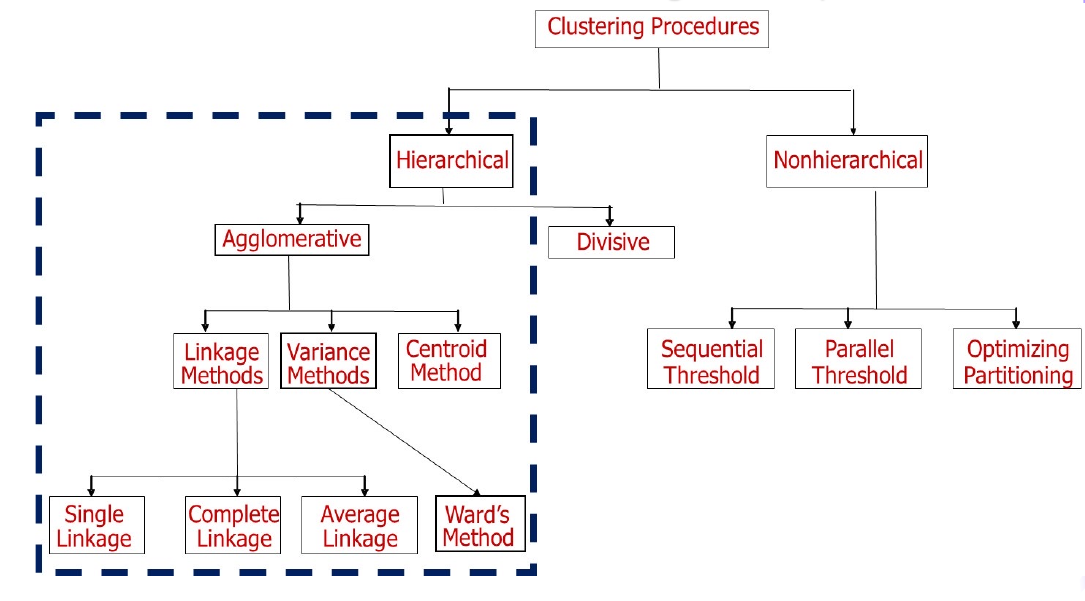
\includegraphics[width=.8\textwidth]{img/chapter-3/clustering-graph.png}
\caption{Esempio di clustering gerarchico}\label{img:clustering-graph}
\end{figure}

Fatta una paronamica generale sul clustering, ai fini del corso, andremo a concentrarci sul clustering gerarchico agglomerativo. Partendo dal considerare il \textbf{clustering gerarchico}, esso può essere di due tipi:
\begin{itemize}
    \item \textbf{Agglomerativo}: Si parte dall'avere un cluster per ogni componente, e poi si prosegue agglomerando i cluster fino a che non si ottiene un unico cluster
    \item \textbf{Divisivo}: Si parte da un cluster in cui sono contenutre tutte le compoenti e si prosegue dividendo i vari cluster secondo particolari metodi.
\end{itemize}

Il clustering \textbf{gerarchico agglomerativo} è una tipologia di clustering che parte dall'avere tanti cluster (uno per ogni componente), e poi si occupa di andare ad agglomerare tali cluster in base a particolari metriche. Tali metriche si basano su concetti differenti di definizione di similarità, e per ognuno ci sono varie considerazioni da fare. Le tecniche principali di clustering agglomerativo sono:
\begin{itemize}
    \item \textbf{Linkage Methods}: Vado a collegare i vari cluster in base alla metrica di distanza che vige tra di loro. Dato che non posso valutare la distanza di tutti i punti si può andare a considerare una metrica differente basandosi su diverse e particolari componenti del cluster:
    \begin{itemize}
        \item \textbf{Single Linkage}: Vado a definire la metrica di distanza tra due cluster come la più piccola distanza tra due punti dei cluster (la distanza dei punti più vicini tra due cluster) [\ref{img:single-linkage}]
        \item \textbf{Complete Linkage}: Vado a definire la metrica di distanza come la distanza maggiore tra due punti di un cluster [\ref{img:complete-linkage}]
        \item \textbf{Average Linkage}: Vado a definire la metrica di distanza come la distanza media dei punti tra due cluster [\ref{img:average-linkage}]
    \end{itemize}

    \item \textbf{Centroid Methods}: Molto simile ai metodi linkage, ma al postro di considerare le istanze direttamente appartenenti al cluster, si va a considerare il centroide del cluster (la media dei punti appartenenti al cluster) e si va a valutare la distanza tra i centroidi dei vari cluster (il centroide non è detto che faccia parte degli elementi del cluster)

    \item \textbf{Variance Methods}: Tale metodo cerca di minimizzare la varianza intra-cluster e cerca di massimizzare la varianza inter-cluster. L'utilizzo effettivo di tale metodo ricade nell'utilizzo del metodo di Ward, che cerca di minimizzare la somma delle varianze all'interno di ogni cluster. A livello formale quello che si va a fare è calcolare la distranza tra due cluster mediante l'utilizzo della distanza euclidea quadrata tra i centroidi dei due cluster, pesata per il numero di elementi che compongono i due cluster. La formula è la seguente:
    Dato il cluster \(P\) ed il cluster \(Q\), il calcolo della distanza mediante il \textbf{metodo di Ward} è:
    \[
    d(P,Q) = 2\frac{|P||Q|}{|P| + |Q|}||(\overline{x}_{P},\overline{x}_{Q})||^2
    \]
    Dove \(|P|\) e \(|Q|\) sono il numero di elementi che compongono i cluster \(P\) e \(Q\), mentre \(\overline{x}_{P}\) e \(\overline{x}_{Q}\) sono i centroidi dei cluster \(P\) e \(Q\).
\end{itemize}

\begin{figure}[h]
\centering
\begin{subfigure}[b]{0.8\textwidth}
\centering
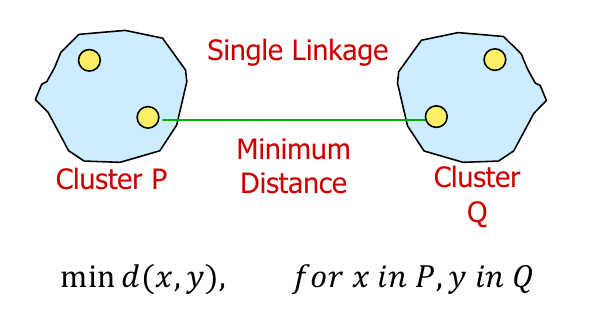
\includegraphics[width=\textwidth]{img/chapter-3/single-linkage.png}
\caption{Single Linkage}\label{img:single-linkage}
\end{subfigure}

\hfill

\begin{subfigure}[b]{0.8\textwidth}
\centering
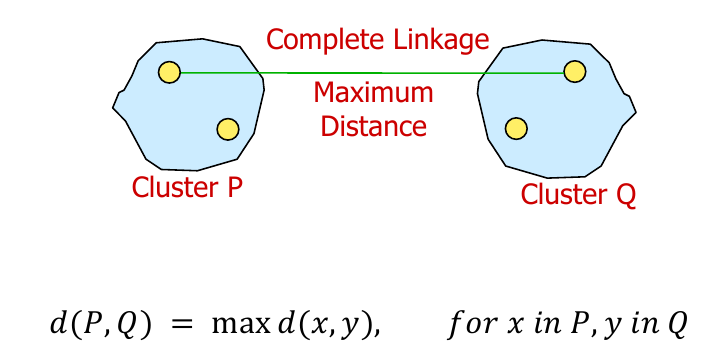
\includegraphics[width=\textwidth]{img/chapter-3/complete-linkage.png}
\caption{Complete Linkage}\label{img:complete-linkage}
\end{subfigure}

\hfill
\begin{subfigure}[b]{0.8\textwidth}
\centering
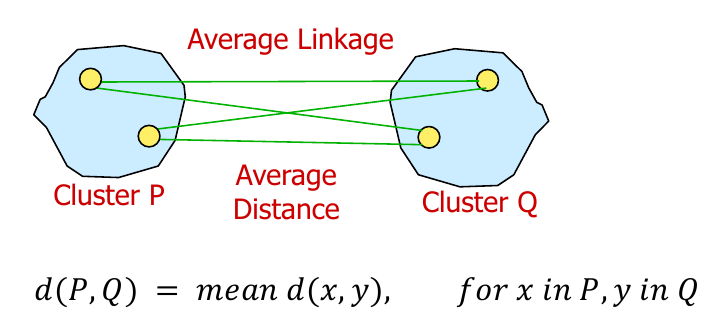
\includegraphics[width=\textwidth]{img/chapter-3/average-linkage.png}
\caption{Average Linkage}\label{img:average-linkage}
\end{subfigure}

\caption{Tipi di metriche per il Linkage Clustering}
\end{figure}

In generale, quindi, un algoritmo di clustering gerarchico agglomerativo segue i seguenti passi:

\begin{enumerate}
\item Calcolo della matrice di distanza tra tutte le componenti date in input
\item Impostare ogni componente come un cluster a se stante
\item Ripetere fino a che non rimane un solo cluster:
\begin{itemize}
    \item Trovare i due cluster più vicini secondo la metrica di distanza scelta ed unirli in un unico cluster
    \item Aggiornare la matrice di distanza per tenere conto del nuovo cluster
    \item Ripeti fino a che non rimane un solo cluster
\end{itemize}
\end{enumerate}
\clearpage

La parte in cui incidono di più le decisioni dei criteri di distanza (linkage, centroid, variance) è nella parte di calcolo della distanza dell'algoritmo. Ad ogni possibile metodo utilizzato, viene associato un diverso modo di calcolare la matrice di distanza, e di conseguenza, si avrà una diversa struttura del clustering finale.
La scelta su quali cluster agglomerare rimane la stessa, ovvero si agglomerano i cluster con la distanza minore tra loro. (questo accade per tutti i metodi, tale metodo di scelta di agglomerazione prescinde dalla metrica utilizzata per calcolare la distanza tra i cluster [che invece contiene una serie di criteri di scelta precedentemente discussi]).

La parte più importante di un clustering gerarchico è il fatto che poi alla fine si va a ricavare un legame tra i vari cluster, che può essere rappresentato mediante un dendogramma. Un dendogramma è un grafo aciclico orientato, dove il nodo rappresenta il cluster "finale" (intero dataset), le foglie sono i singoli elementi, ed i nodi, sono i cluster che nel processo sono stati agglomerati. La comodità di avere un dendogramma è che si può andare a "tagliare" il grafo ad un certo livello, ottenendo così un numero di cluster desiderato. (guardare figura [\ref{img:dendogramma}]). Quado vado a scegliere il livello a cui tagliare il dendogramma, mediante la larghezza del dendogramma, riesco a capire se due cluster se hanno una varianza più bassa o più alta. Più sono vicino alla radice, meno sono i cluster, ma la similarità intra-cluster si riduce. Mentre, più sono vicino alle foglie, più sono i cluster, e la similarità intra-cluster aumenta. 

\begin{figure}[h]
\centering
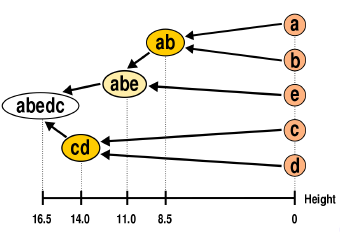
\includegraphics[width=.8\textwidth]{img/chapter-3/dendogramma.png}
\caption{Esempio di dendogramma}\label{img:dendogramma}
\end{figure}

\begin{warn}
In base al metodo utilizzato si avrà una clusterizzazione differente. Quindi la scelta del metodo di calcolo della distanza è fondamentale per ottenere un buon risultato finale.
\end{warn}

\subsubsection{Interpretazione del clustering}
Alla fine del clustering, tutte le componenti facenti parte dell'insieme di dati in ingresso sono associati ad un singolo cluster. In generale posso eliminare i cluster poco influenti (che occupano poche risorse) e che hanno una dimensione molto piccola (poche componenti) [Attenzione, le regole precedentemente presentate per la selezione di un cluster non possono essere divisie, devono essere entrambe vere, altrimenti si potrebbe ricadere in errori di valutazione]. Ottenuti i cluster, si cerca di interpretarli in maniera funzionale (in baso alla tipologia di dato che si sta andando a valutare).

Una volta ottenuti e valutati i cluster si va a trovare un singolo valore rappresentativo per ogni cluster, ciò ci permetterà di poter rappresentare il workload mediante un minor numero di componenti.

I cluster tra loro devono essere quanto più dissimili possibile, mentre le componenti all'interno di un cluster devono essere quanto più simili possibile tra di loro. In statistica possiamo definire tale concetto parlando di varianza; più precisamente si enuncia che:
\textit{La varianza intra-cluster dev'essere quanto più piccola possibile, mentre la varianza inter-cluster dev'essere quanto più grande possibile.}
L'unico problema legato all'utilizzo della varianza è che non rispetta la disuguaglianza triangolare, e pertanto non può essere utilizzata come metrica di distanza per il clustering. Pertanto si utilizza la devianza come metrica per valutare la bontà del clustering effettuato, questo perchè rispetta la disuguaglianza triangolare:
\[
devianza\_totale = devianza\_intra\_cluster + devianza\_inter\_cluster
\label{for:triangolare}
\]

In maniera più formale, ci è richiesto un metodo per valutare tali devianze. Per valutare la devianza intra-cluster si utilizza la seguente formula:

Dati \(n\) oggetti in uno spazio vettoriale \(d\)-dimensionale\\ \(X_i = (x_{i1}, x_{i2},\dots, x_{id})\), \(\forall i \in [1,n]\), si definisce devianza intra-cluster:

\[
intra\_cluster\_deviance = \sum_{k=1}^{K}\sum_{i=1}^{n_k}||X_i - \overline{X}_k||^2
\]

Dove:
\begin{itemize}
\item \(\overline{X}_k = \frac{1}{n_k}\sum_{C(i)=k}X_i\): Centroide del cluster \(k\)
\item \(n_k\): Numero di oggetti nel cluster \(k\)
\item \(||X_i - X_j||^2 = \sum_{p=1}^{d}(x_{ip} - x_{jp})^2\)
\item \(K\): Numero di cluster che si vanno a considerare
\end{itemize}

Mentre per valutare la devianza inter-cluster si utilizza la seguente formula:

Dati i \(K\) cluster e \(\overline{X}\) media di tutti gli elementi. Si definisce la devianza inter-cluster come:
\[
inter\_cluster\_deviance = \sum_{k=1}^{K}n_k||\overline{X}_k - \overline{X}||^2
\]

Dove (formalmente):
\begin{itemize}
\item \(\overline{X} = \frac{1}{n}\sum_{i=1}^{n}X_i\): Media di tutte le componenti date in ingresso all'algoritmo
\item \(n\): il numero di componenti dati in ingresso all'algoritmo
\end{itemize}

Si può dimostrare che la varianza intra-cluster e la varianza inter-cluster rispettano la disuguaglianza triangolare (vedi formula [\ref{for:triangolare}])

\subsection{Valutazione della devianza persa}
Quando vado ad effettuare la sintetizzazione del workload mediante l'utilizzo di PCA + clustering, devo valutare la quantità di devianza persa. La devianza persa è la quantità di devianza che non viene più rappresentata dalle componenti selezionate per rappresentare il workload. Per calcolarla, vado a valutare i seguenti valori:
\begin{itemize}
    \item \textbf{Varianza persa PCA}: La devianza portata dai parametri che non sono stati selezionati dopo la PCA
    \item \textbf{Varianza persa Clustering}: La devianza intra-cluster, ovvero la devianza che non viene più rappresentata dalle componenti selezionate per rappresentare il workload
\end{itemize}

Per il calcolo della devianza totale persa vado a considerare la seguente formula:
\[
devianza\_persa = devianza\_persa\_PCA + (devianza\_guadagnata\_PCA * devianza\_intra\_cluster)
\]

Oppure in maniera identica posso utilizzare la formula:
\[
devianza\_persa = 1 - (devianza\_guadagnata\_PCA * devianza\_inter\_cluster)
\]

In questo secondo caso sono andato a valutare prima la quantità effettiva di varianza "guadagnata" tra i due processi e poi ho sottratto ad 1 (essendo tutto espresso in percentuali).

Esempio:\\
Una volta effettuata la PCA con la selezione dei parametri sul mio workload ho che la devianza considerata è del \(95\%\).\\
Poi facendo il clustering, scopro che la mia devianza intra-cluster è pari al \(10\%\) e di conseguenza quella inter-cluster è pari al \(95\%\).\\
Di conseguenza posso calcolare la devianza totale persa come:
\[
devianza\_persa = devianza\_persa\_PCA + (devianza\_guadagnata\_PCA * devianza\_intra\_cluster)=
\]
\[
= 0.05 + (0.95 * 0.10) = 0.145 = 14.5\%
\]

Se vado a calcolare tale valore con l'altra formula, ottengo:
\[
devianza\_persa = 1 - (devianza\_guadagnata\_PCA * devianza\_inter\_cluster)=
\]
\[
= 1 - (0.95 * 0.90) = 1 - 0.855 = 0.145 = 14.5\%
\]

Notiamo come i due valori siano esarramente uguali.

\begin{info}
\textit{Tale dimostrazione è stata aggiunta solo a scopo didattico e non è richiesta ai fini dell'esame}
Il collegamento tra i due calcoli è molto semplice e risulta dimostrabile. Per dimostrare tale collegamento si può procedere nel seguente modo (consideriamo la deviazione guadagnata dalla pca denotata come dgp, mentre la deviazione persa dalla pca dpp, mentre poi vado a considerare la deviazione intra-cluster come dic, mentre la deviazione inter-cluster dec). Posso dimostrare tale legame nel seguente modo:
\[
deviazione_persa = dpp + (dgp * dic) = 1 - dgp + (dgp * dic)=
\]
\[
= 1 - (1 - dic) * dgp = 1 - dec * dgp
\]
Come possiamo vedere alla fine siamo arrivati alla seconda forma di calcolo della devianza persa totale
\end{info}

\subsection{Modelli di Markov}
Un \textbf{modello di Markov} è una tipologia di modello in cui uno stato successivo o prossimo, dipende solamente dallo stato corrente. Esso può essere rappresentato, quindi, mediante l'utilizzo di un grafo. Un modello di markov, quindi, ha un modo di decidere il prossimo stato (che dipenderà solo da quello attuale). La possibilità di raggiungere un dato stato considerato lo stato precendente viene chiamata \textbf{Probabilità di transizione}, mentre la tabella con tutte le probabilità di raggiungere uno stato dato lo stato corrente, è detta \textbf{Matrice delle transizioni} (in inglese sarebbe matrice di transizione, ma tale definizione collide con le conoscenze precedenti di algebra e geometria). Tale tipologia di modello permette di trovare dei "pattern" o path, che vengono seguiti durante "l'utilizzo" di un applicativo (workload). Permettendo di andare a stressare il sistema su quelle operazioni che si sanno sono più ripetute (probabili). La stima della tabella delle transizioni è fatta tramite un'approccio di tipo frequentista


\chapter{Caratterizzazione di Dati Misurati}
Resi noti una serie di dati misurati, quello che si vuole andare a fare è trovare un modello statistico che mi permetta di avere un'approssimazione valida di tali dati. Ci sono varie tipologie di tecniche e di approcci. Per grandi quantità di dati si farà un utilizzo massiccio della \textbf{Statistica inferenziale}, che comprende tutta una serie di metodi che permettono di andare a stimare un modello quantò più opportuno possibile ai dati che si stanno andando ad analizzare

\subsection{Media, Mediana e Moda}
Dato un insieme di dati, si possono andare a valutare 3 valori principali (e scalari), che ci permettono di approssimare (in maniera grossolana), la nostra distribuzione di dati (rappresentabile, anche, mediante un istogrammma). I valori a cui si fa riferimento sono:
\begin{itemize}
    \item \textbf{Media}: Media statistica di tutti i valori che si sta andando a considerare. Se si ha un set di valoi \(X = (x_1,x_2,\dots,x_n)\), allora definiamo come media:
    \[
    \overline{X} = \frac{1}{n}\sum_{i=1}^{n}x_i
    \]
    La media, però, non tiene conto dell'asimmetria dei dati (skewness), quindi se ad esempio un sistema ha dei tempi di ripsosta sempre stabili, e poi, un singolo caso di tempo di risposta lungo, potrebbe avere la stessa media di un sistema che ha mediamente tempi di risposta più lunghi (molto sensibile ad eventuali comportamenti limite)
    \item \textbf{Mediana}: La mediana di un set di valori \(X = (x_1,x_2,\dots,x_n)\) è data dalla selezione del valore centrale del set di valori ordinati. Per capire, si ordina il set di valori \(X\) e poi si seleziona l'elemento presente in \(\left\lfloor\frac{n}{2}\right\rfloor\). Ciò però presenta un problema, se il numrero di valori è dispari allora io seleziono l'unica posizione centrale presente (es. Se ho 3 elementi seleziono 1), mentre se ho un valore pari devo trovare un modo con cui scegliere quale elemento considerare, pertanto, essendo due i valori centrali, se ne fa la media (es. se ho 4 elementi, farò la media del valore in posizione 1 ed in posizione 2). La mediana a differenza della media viene presa direttamente dai valori reali e non calcolata considerando tutti i valori, ciò gli permette di essere più resistente agli outlier e sopratutto a distribuzioni asimettriche (resistente alla skewness)
    
    \item \textbf{Moda}: La moda rappresenta il valore più probabile all'interno di una distribuzione (quello presentato più volte). Di conseguenza tiene conto del picco presente nell'istrogramma. Il problema della moda è che può non esistere (caso di distribuzioni uniformi), oppure può assumere più di un valore (immaginare una distribuzione bi-gaussiana). Nonostante le considerazioni precedenti, la media è totalmente immune agli outlier (vedo solo il più probabile), e mi permette di evitare anche le ambiguità di una particolare distribuzione
\end{itemize}

\begin{info}
Nella descrizione dei parametri precedenti si è parlato di asimettrie dei dati (skewness dei dati), tale valore per piccole quantità di campioni può essere approssimato con la formula:
\[
skewness = \frac{y_{max}}{y_{min}}
\]
Da tale formula comprendo che più il valore è alto e più i dati sono "asimettrici". Ma tale considerazione è più corretta quanto più è piccola la quantità di campioni che sto andando a considerare 
\end{info}


Un semplice criterio per decidere quale tipologia di metrica utilizzare è quella mostrata in figura [\ref{img:criterio-media-mediana}]

\begin{figure}[h]
\centering
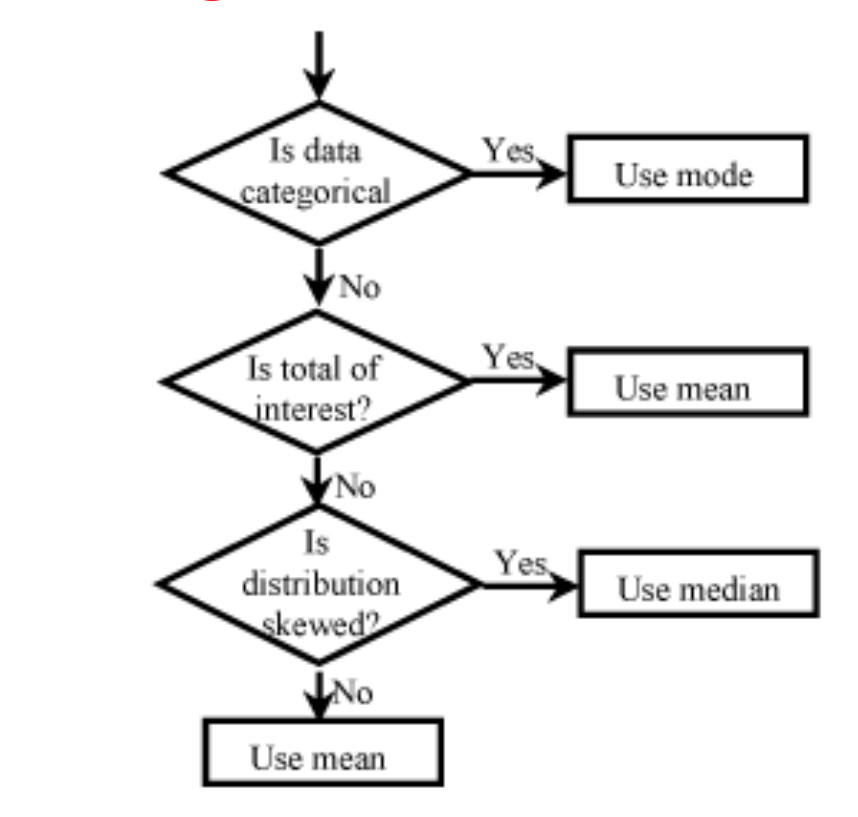
\includegraphics[width=.5\textwidth]{img/chapter-4/criterio-media-mediana.png}
\caption{Semplice schema di un criterio per la scelta della metrica da utilizzare}\label{img:criterio-media-mediana}
\end{figure}

I valori descritti, oltretutto, possono essere ottenuti osservando anche la distribuzione dei dati mediante degli istogrammi di occorrenza. In questo modo è anche più facile campire quale metrica sia meglio utilizzare.

\begin{figure}[H]
\centering
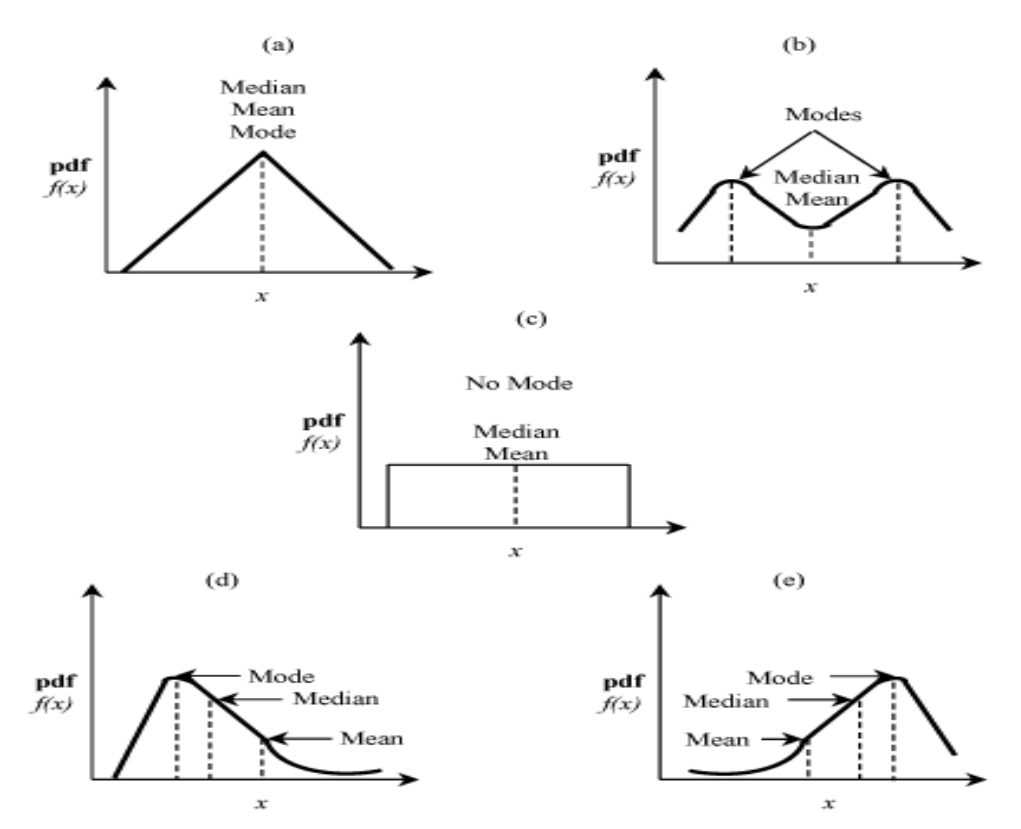
\includegraphics[width=.5\textwidth]{img/chapter-4/grafici-media-mediana.png}
\caption{Grafici illustrativi dei parametri discussi}\label{img:grafici-media-mediana}
\end{figure}

\subsection{Indici di dispersione}
Andare ad approssimare una distribuzione di valori con un singolo valore non basta, tale informazione non mi permette di considerare anche la \textbf{variabilità} che i dati possono avere nel tempo.
Uno strumento utile per avere un'idea della variabilità, sono gli \textbf{indici di dispersione}. Tra le metriche più utilizzate possiamo trovare:
\begin{itemize}
\item \textbf{Range}: Il range è un parametro molto basilare che viene calcolato come: \(v_{max} - V{min}\). Tale metrica, per quanto semplice, è anche molto poco resistente agli outlier
\item \textbf{Varianza campionaria (o deviazione standard)}: Tale parametro è strettamente calcolato dai dait e dipende dalla loro distribuzione
\item \textbf{10- e -90 Percentile}: Prendendo una distribuzione di dati si vanno a considerare due valori:
\begin{itemize}
    \item \textbf{\(P10\)}: Valore dei dati sotto il quale cade il 10\% dei dati considerati
    \item \textbf{\(P90\)}: Valore dei dati sotto il quale cade il 90\% dei dati considerati (quindi solo il restante 10\% è maggiore)
\end{itemize}
Si definisce poi come indice di dispersione il range calcolato su tali valori: \(range = P90-P10\). Se vediamo tali valori in riferimento alla pdf dei dati (il loro istogramma) e alla CDF. Si ha che per calcolare il valore P90 e P10, vado a valutare il valore della CDF in base al percentile ricercato (\(F(x_p) = 0.10\) o \(0.90\)), oppure, nel caso della pdf vado a calutare l'integrale (guardare la relazione tra CDF e pdf)\(\left [\int_{-\infty}^{x_p}f(x)dx = 0.10 | 0.90\right ]\). Il percentile solitamente può essere chiamato anche \textbf{quartile}. La differenza sta nella notazione, per il quartile si dice \(0.1\)-quartile (\(\alpha\)-quartile), mentre il percentile si esprime come 10-percentile (\(100*\alpha\)-percentile). Per stimare tali valori su un insieme di dati discreto (quindi non distribuzioni continue su cui effettuare integrali o derivate), posso andare ad effettuare, prima un ordinamento e poi a selezionare uno specifico valore in base alla \(\alpha\) scelta. Precisamente si va a selezionare il valore in posizione: \([(n-1)*\alpha + 1]\)

\item \textbf{Semi Inter-Quartile Range}: Tale metrica va ad utilizzare la definizione di due particolari casi di quartile. Più precisamente si va a considerare i quartili: \(0.75\)-quartile (75-percentile) [o terzo quartile] ed il \(0.25\)-quartile (25-percentile) [o primo quartile]. Tali valori sono poi combinati e si va a calcolare il valore del Semi Inter-Quartile Range come:
\[
SIQR = \frac{Q_3 - Q_1}{2}
\]

\item \textbf{Mean Absolute Deviation}: Vado a considerare la somma delle deviazioni, ma che sia sottoposta prima all'operazione di modulo, in modo da evitale l'azzeramento della somma delle deviazioni (come visto nel capitolo precedente). La formula è la seguente:
\[
MAD = \frac{1}{n}\sum_{i=1}^{n}|x_i - \overline{x}|
\]
Dove \(\overline{x}\) è la media dei valori: \(x_1,x_2, \dots, x_n\).

\end{itemize}

Un elemento utile quando si sta guardando il grafico dei dati è il \textbf{boxplot}. Il boxplot ci da un informazione grafica iniziale su dove i valori di interesse per il calcolo delle diverse metriche si trovino. Principalmente ci permette di poter osservare le seguenti metriche [\ref{img:boxplot}]:
\begin{itemize}
    \item \textbf{Valore massimo}
    \item \textbf{Valore minimo}
    \item \textbf{Mediana}(o 0.5-quartile/secondo quartile)
    \item \textbf{Primo Quartile}(0.25-quartile)
    \item \textbf{Terzo Quartile}(0.75-quartile)
    \item \textbf{Semi Inter-Quartile Range}
\end{itemize}

\begin{figure}[H]
\centering
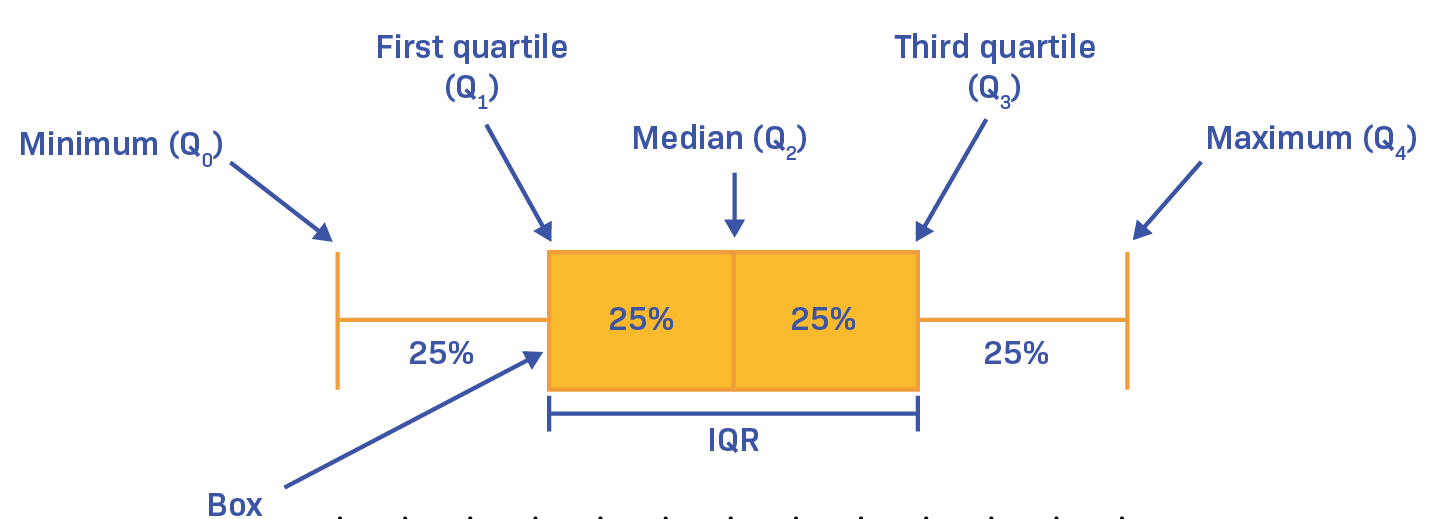
\includegraphics[width=.7\textwidth]{img/chapter-4/boxplot.png}
\caption{Struttura di un boxplot}\label{img:boxplot}
\end{figure}

La stima dell'indice di dispersione è qualcosa di complicato, sopratutto quando ci sono in mezzo gli outlier. Pertanto, solitamente, come metrica al posto della varianza (che non è completamente immune agli outlier), si preferisce utilizzare il Semi Iter-Quartile Range (SIRQ), che è più resistente alla presenza di outlier (anche più di qualcuno). Mentre come metrica centrale si preferisce l'uso della mediana, questo poichè ci è assicurato che esista (a differenza della moda), e sopratutto che faccia parte dell'insieme di valori considerato (diversamente dalla media). Questo spiega anche la costruzione del boxplot e dei valori che va a mettere in evidenza.

\subsection{Quantile-Quantile Plot}
Il \textbf{Quantile-Quantile Plot} è un metodo che ci permette di confrontare se due popolazioni hanno una distribuzione simile o meno. Nel nostro caso lo si utilizzerà per confrontare la distribuzione della nostra popolazione rispetto alla distribuzione normale.
La composizione di base di un grafico quantile-quantile generico è la seguente:
Si va a definire un punto \(p\) come \(p = (x_i, y_i)\), dove \(x_i\) è il valore teorico dell' i-esimo quantile, mentre \(y_i\) è il valore reale dell'i-esimo quantile. Per quanto riguarda i parametri reali non è complicato trovare i quartili (basta utilizzare la specifica formula in base ad \(\alpha\)), mentre per i parametri teorici risulta più complesso dato che bisogna trovare il modo di invertire la CDF. Per ricavare i valori della normale (funzione gaussiana di media nulla e varianza unitaria). Vado a calcolare il quartile come: \(q_i = \frac{i-0.5}{2}\), da cui posso ricavare il valore teorico come: \(x_i = 4.91\left [ q_i^{0.14} - (1-q_i)^{0.14} \right ]\).
Quindi, in generale, data una popolazione posso plottare il grafico utilizzando le metriche esposte in precedenza, e confrontare la distribuzione dei dati reali con quelli di una normale. In questo modo cerco di capire quanto la distribuzione della popolazione sia simile ad una distribuzione gaussiana. Alcuni esempi sono mostrati alla figura: [\ref{img:qqplot}]

\begin{figure}[h]

\centering
\begin{subfigure}[b]{0.5\textwidth}
\centering
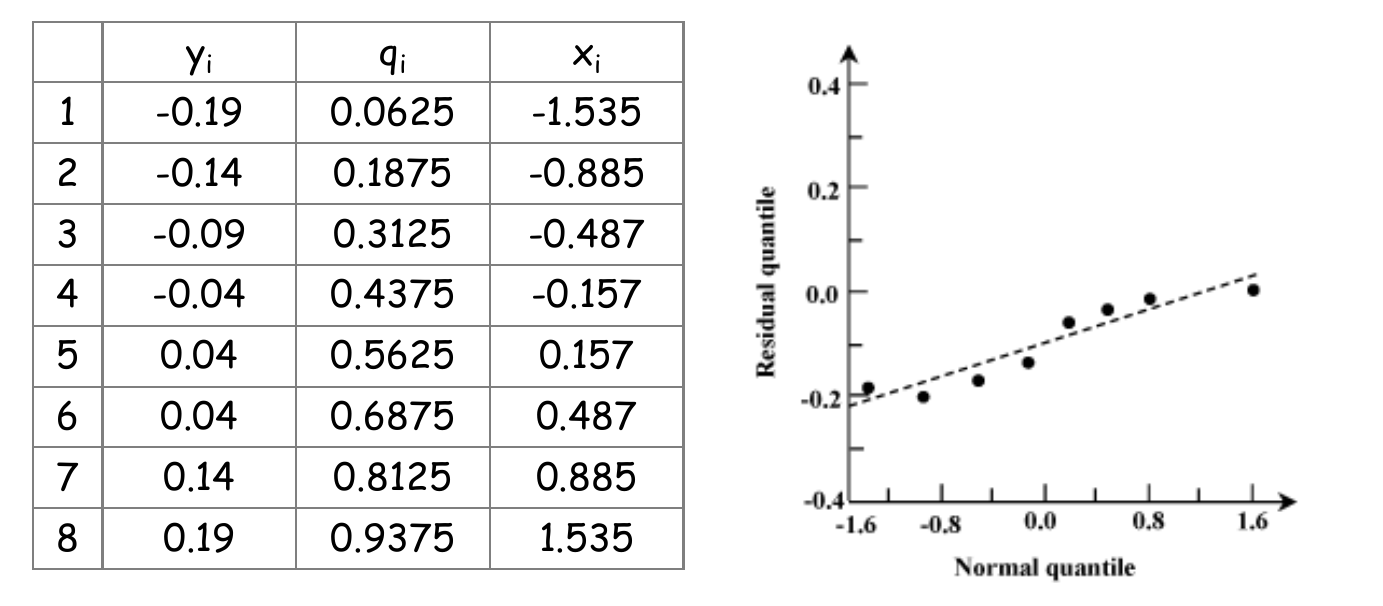
\includegraphics[width=\textwidth]{img/chapter-4/qqplot-ex.png}
\caption{Esempio di Quantile-Quantile plot rispetto alla normale}\label{img:qqplot-ex}
\end{subfigure}

\hfill

\begin{subfigure}[b]{0.6\textwidth}
\centering
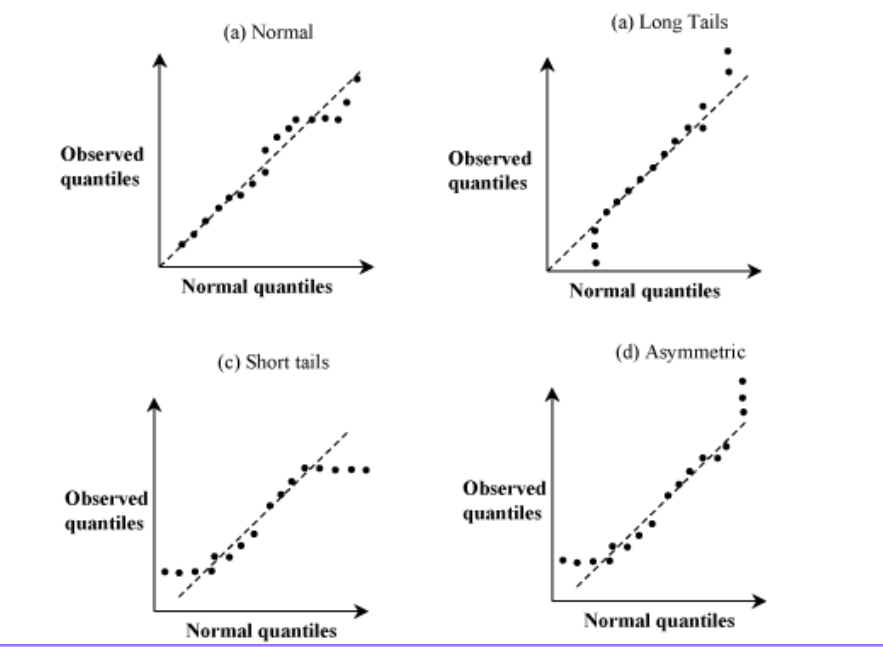
\includegraphics[width=\textwidth]{img/chapter-4/qqplot-confronto.png}
\caption{Diverse tipologie di rappresentazioni in base alla natura della popolazione}\label{img:qqplot-confronto}
\end{subfigure}

\caption{Applicazioni della Quanitile-Quantile plot (o  rappresentazione Quantile-Quantile)}\label{img:qqplot}
\end{figure}

\clearpage
\subsection{Intervalli di confidenza e dimensione del campionamento}
Solitamente, andare a considerare tutta la popolazione, potrebbe essere oneroso, pertanto, si potrebbe considerare di fare delle valutazioni su un numero minore di componenti estratte in maniera randomica (campionamento della popolazione). La problematica principale risiede nelle assunzioni che si potrebbe fare sulle statistiche della popolazione intera, ovvero, calcolare qualche valore per l'intera popolazione a partire dalla popolazione intera. Tali metodoligie sono sotto il nome di \textbf{statistica inferenziale}.
Per comprenderne bene il legame osservare l'immagine [\ref{img:statistica-inferenziale}].

\begin{figure}[h]
\centering
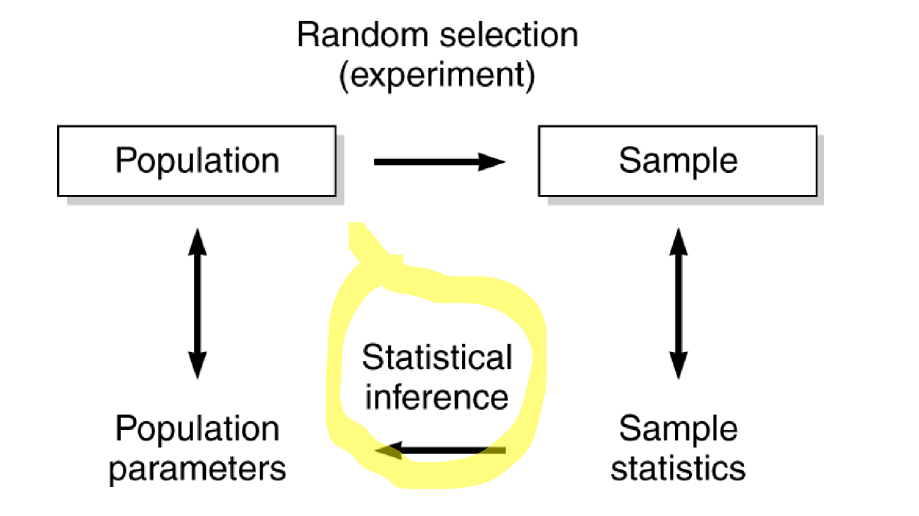
\includegraphics[width=.7\textwidth]{img/chapter-4/statistical-inference.png}
\caption{Collocazione logica della statistica inferenziale}\label{img:statistica-inferenziale}
\end{figure}

\subsubsection{Campioni e Popolazione}
\uppercase{è} importante definire cosa si intende quando si sta parlando di popolazione o di campioni, ciò ci permetterà di poter definire tutta una serie di principi statistici, utili, per effettuare l'inferenza statistica.
Formalmente si definisce \textbf{popolazione} l'insieme totale di tutte le componenti (o istanze), mentre si definisce \textbf{Campione}(O Sample), un insieme di n osservazioni provenienti dai campioni. In generale è importante, definire anche il significato di \textbf{parametri}, i dati associati alla popolazione, essi saranno indicati con le lettere greche (ad esempio la media e la varianza associate alla popolazione, tali valori per qualunque saranno i campioni estratti, non varieranno [saranno costanti]); mentre si definiscono \textbf{statistiche} i valori associati ai sample della popolazione, esse saranno rappresentate da lettere comuni (tali valori variano da campione a campione e quindi non sono costanti).

\begin{info}\label{inf:distribuzioni-Campionarie}
\textit{Tale pezzo non è richiesto ai fini dell'esame ma potrebbe essere utile in una fase di approfondimento e studio della statistica inferenziale}
    \\
\textbf{Distribuzioni Campionarie}\\
Si definisce \textbf{Distribuzione Campionaria}, una distribuzione di probabilità associata alla variabile aleatoria \(\overline{X}\), che è la composizione di diverse osservazioni \(X_1, X_2, \dots, X_n\) che sono ricavate da k-campioni della popolazione iniziale. \(\overline{X}\) non è altro che una variabile aleatoria associata alla media delle osservazioni (media campionaria).
\begin{warn}
Quando parliamo di \(\overline{X}\) stiamo parlando della variabile aleatoria (quindi un valore casuale), mentre la distribuzione campionaria è la funzione di distribuzione di probabilità(pdf) associata ad \(\overline{X}\)
\end{warn}

Pertanto, possiamo definire \(\overline{X}\) come:
\[
\overline{X} = \frac{X_1 + X_2 + \dots + X_n}{n}
\]
Da cui, applicando il \textbf{teorema fondamentale della media}, si ottiene che:
\[
E(\overline{X}) = \frac{E(X_1) + E(X_2) + \dots + E(X_n)}{n}
\]
Andando a considerare un caso più semplice, dove la popolazione ha media nota e pari a \(\mu\) e varianza \(\sigma^2\), e dove le variabili aleatorie \(X_1, X_2, \dots, X_n\), associate alle osservazioni dei campioni, sono delle variabili aleatorie indipendenti ed identicamente distribuite (sono la stessa variabile aleatoria con media \(\mu\) e varianza \(\sigma^2\), allora si può dire che:
\[
E(\overline{X} = \frac{\mu + \mu + \dots + \mu}{n} = \mu)
V(\overline{X}) = E((\overline{X} - \mu)^2) = \frac{\sigma^2 + \sigma^2 + \dots + \sigma^2}{n^2} = \frac{\sigma^2}{n} 
\]
Da tali formule si sono ricavati dei valori associati alla distribuzione campionaria, dette statistiche. Com'è possibile notare, più la dimensione del sample size cresce e più la varianza diminuisce, ciò ci fa capire che l'errore fatto sulla media diminuisce man mano (base per la valutazione dello standard error).
Andando ad invalidare le ipotesi fatte sulla struttura della popolazione (sulla sua distribuzione di probabilità), allora si può andare a valutare il \textbf{Teorema del limite centrale}.
\end{info}

\subsubsection{Standard Error}
Quando vado a valutare le statistiche riferite ai vari campioni presi dalla popolazione, con sample size pari ad n, voglio capire quanto queste siano effettivamente vicine a quelle reali. La problematica risiede proprio nel calcolo dei parametri. Di base, non si possono fare delle assunzioni sulla distribuzione di probabilità della popolazione (solitamente non è gaussiana, ma ha una forma generica o skewed (ambigua)). Pertanto non posso andare a valutare la varianza campionaria, questo poichè non posso fare assunzioni. Pertanto, in questi casi, ci viene in aiuto il \textbf{teorema del limite centrale}.
Il \textbf{teorema del limite centrale} ci dice che:
\\\textbf{Ipotesi}\\
Siano \(X_1, X_2, \dots, X_n\), n-variabili aleatorie Indipendenti ed identicamente distribuite (hanno tutte la stessa distribuzione, poichè la loro base dei dati è la stessa)
\\
Sia la sample size n, un valore orientativamente grande \(n>=30\)
\\
\textbf{Tesi}
\\
Allora posso dire che la \textbf{distribuzione campionaria} della media (distribuzione della variabile aleatori \(\overline{X}\)), è riconducibile ad una funzione normale con:
\begin{itemize}
    \item \textbf{Media} pari a \(\mu\) (media della popolazione)
    \item \textbf{Varianza} pari a \(\frac{\sigma^2}{n}\) (o deviazione standard \(\frac{\sigma}{\sqrt n}\))
\end{itemize}

\begin{info}
\textit{Tale pezzo non è richieto per lo svolgimento dell'esame, ma solo al fine di approfondire alcuni concetti}
\\
Seguendo quello che si è visto nel precedente approfondimento [\ref{inf:distribuzioni-Campionarie}]; Il teorema del limite centrale non è altro che la conseguenza della composizione della variabile aleatoria \(\overline{X}\), rispetto alle variabili aleatorie associate ai campioni. Se le variabili aleatorie sono indipendenti (ce lo assicurano le indipendenze tra le varie osservazioni) ed identicamente distribuite (il fatto che le varie variabili abbiano la stessa pdf(e quindi non lo stesso valore), ci assicura, che la  media di tutte le distribuzioni sia \(\mu\)), allora il teorema del limite centrale non è altro che la dimostrazione del caso particolare che si è mostrato in precedenza. Se si vuole avere una maggior formalità nell'esporre il teorema del limite centrale si può andare a definire, una nuova variabile aleatoria \(Z\), come:
\[
Z = \frac{\overline{X} - \mu}{\sigma / \sqrt{n}} 
\xrightarrow{\,n \to \infty\,} 
\mathcal{N}(0,1)
\]
\end{info}
\chapter{Modelli di Regressione}
Un \textbf{Modello di regressione}, permette di poter valutare il valore di una variabile come funzione di ulteriori altre variabili. Per essere precisi, si definiscono:
\begin{itemize}
    \item \textbf{Response variables}: Le variabili che vengono stimate dal modello
    \item \textbf{Predictor variables}(o predictors o factors): Variabili utilizzare per andare a valutare le Response variables
\end{itemize}
I modelli regressivi possono essere di due principali tipologie:
\begin{itemize}
    \item \textbf{Lineare}: Modelli più utilizzati nella pratica. In generale vanno ad utilizzare tutti i parametri, ma molto spesso (ed anche in questo corso), si possono considerare dei modelli che si basano su un singolo predictor variable, tali modelli sono più semplici e vengono chiamati \textbf{simple linear regression models} 
    \item \textbf{Non Lineare}: Modelli non molto utilizzati che fanno uso delle relazioni non lineari tra le predictor variables
\end{itemize}

Oltre ad andare a definire i modelli e la loro struttura, bisogna definire quanto un modello sia qualitativamente buono rispetto ai dati utilizzati, quindi bisogna definire delle metriche di \textbf{qualità del modello}. Tali tecniche permettono di capire se il modello trovato è affine ai dati utilizzati per calcolarlo. Più precisamente, possiamo avere due tipologie di approcci al seguente problema:
\begin{itemize}
    \item \textbf{Approccio visuale}: Si va a valutare il modello in base a quanto questo sia "chiuso" rispetto ai valori considerati (quanto questo approssimi bene l'andamento delle mie osservazioni). Per comprendere bene tale concetto si può far riferimento alla figure [\ref{img:error-vision}]
    
    \item \textbf{Valutazione degli errori}: In primis devo capire come andare a definire il mio errore. Il modo più semplice per andarlo a definire è mediante la differenza tra il valore modellato su x (quindi la y calcolata) ed il valore reale rispetto alla variabile x. In genereale, l'errore, in questa modalità, viene definito come la distanza verticale tra il valore osservato e quello calcolato
\end{itemize}

\begin{figure}[h]
\centering
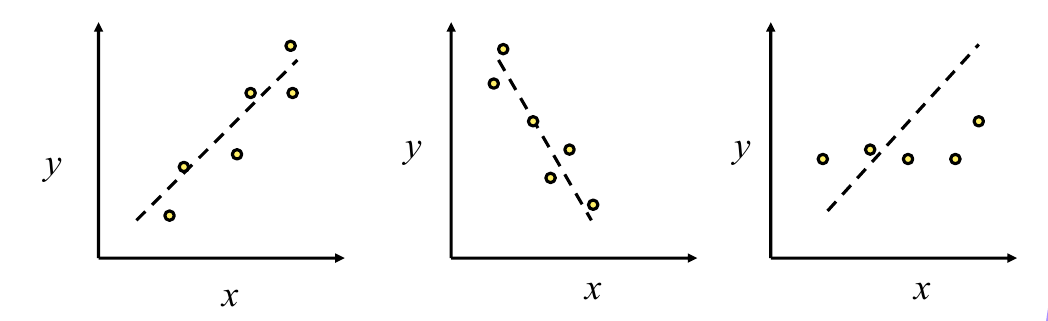
\includegraphics[width=.7\textwidth]{img/chapter-5/quality-regression.png}
\caption{Valutazione visiva dei modelli di regressione lineari}\label{img:error-vision}
\end{figure}

\section{Modelli di regressione lineari semplici}
I \textbf{simple linear regression model}(modelli di regressione lineare semplici), sono dei modelli che hanno un singolo parameter predictor. Queste presupposizione rende più semplice la trattazione di tali modelli, in particolare, il loro calcolo. Per comprendere meglio come si vanno a stimare i parametri del semplice modello lineare, bisogna passare per i \textbf{parametri di qualità del modello}. Più precisamente dalla valutazione dell'errore.  
Andando ad aggiungere più formalismo:\\
Considerando le \(n\) osservazioni: 
    \[(x_1, y_1), (x_2, y_2), \dots, (x_n, y_n)\]
    si va a costruire un modello lineare come: 
    \[\hat{y} = b_0 + b_1*x\]
    basato su tali osservazioni. Per valutare l'errore si prosegue nel calcolo del residuo come:
    \[e_i = y_i - \hat{y}_i\]
Con tale definizione, si può proseguire andando ad imporre la condizione, che la somma di tutti i residui sia pari a 0:
\[
\sum_{i=1}^{n}e_i = \sum_{i=1}^{n}(y_i - \hat{y}_i)=\sum_{i=1}^{n}(y_i - b_0 - b_1*x_i) =  0
\]
Andando a risolvere tale equazione non si troverebbe una \textbf{soluzione univoca}, poichè si avrebbe una equazione in 2 incognite, che quindi ha infinito alla 1 soluzioni. Pertanto vi è richiesto di definire un'ulteriore equazione, ovvero quella che fa riferimento all'\textbf{SSE}(Sum of Squared Error), che dev'essere minimizzato, ed è definito come:
\[
SSE = \sum_{i=1}^{n}e_i = \sum_{i=1}^{n}(y_i - b_0 - b_1*x_i)^2
\]
Questo però è un problema di minimizzazione vincolata, che quindi viene risolto in certi modi utilizzando varie tecniche. Noi utilizzeremo una tecnica pervenuta dall'esame di analisi 1, ovvero andremo a derivare la funzione quadrata e a porla uguale a 1. 

\begin{info}
\textit{Il prof non ha dato molto peso a questa parte, banalizzandola particolarmente. Di seguito, però, si riporta la dimostrazione per il calcolo dei coefficienti b1 e b0}
\\
Partendo dalla media dei residui e ponendola uguale a 0, si ottiene che:
\[
\frac{1}{n}\sum_{i=1}^{n}e_i = \frac{1}{n}\sum_{i=1}^{n}(y_i - b_0 - b_1 * x_i) = \overline{y} - b_0 - b_1 * \overline{x} = 0
\]
Da cui:
\[
b_0 = \overline{y} - b_1*\overline{x}
\]
Andando a sostituire tale definizione nella formula di calcolo dell'errore si avrebbe:
\[
e_i = y_i - \overline{y} + b_1*\overline{x} - b_1 * x_i = (y_i - \overline{y}) - b_1*(x_i - \overline{x})
\]
Qui mi fermo e vado a valutare l'errore quadratico, come:
\[
\frac{SSE}{n-1} = \frac{1}{n-1}\sum_{i=1}^{n}e_i^2 = \frac{1}{n-1}\sum_{i=1}^{n}\left ( (y_i - \overline{y}) - b_1*(x_i - \overline{x}) \right )^2=
\]
\[
= \frac{1}{n-1}\sum_{i=1}^{n}(y_i - \overline{y})^2 + \frac{b_1^2}{n-1}\sum_{i=1}^{n}(x_i - \overline{x})^2 - \frac{2\ b_1}{n-1}\sum_{i=1}^{n}((y_i - \overline{y})*(x_i - \overline{x}))
\]
Andando a denominare \(s_y = \sqrt{\frac{1}{n-1}\sum_{i=1}^{n}(y_i - \overline{y})^2}\), \(s_x = \sqrt{\frac{1}{n-1}\sum_{i=1}^{n}(x_i - \overline{x})^2}\) e \(s_{xy} = \sqrt{\frac{1}{n-1}\sum_{i=1}^{n}((y_i - \overline{y})*(x_i - \overline{x}))}\), si ottiene:
\[
\frac{SSE}{n-1} = s_y^2 + b_1^2 s_x^2 - 2 b_1 s_{xy}^2
\]
Andando a derivare rispetto a \(b_1\) si ottiene:
\[
\frac{1}{n-1}\frac{d SSE}{d b_1} = 2 b_1 s_x^2 - 2 s_{xy}^2 = 0
\]
da cui, si può calcolare \(b_1\) come:
\[
b_1 = \frac{s_{xy}^2}{s_{x}^2} = \frac{\sum_{i=1}^{n}((y_i - \overline{y})*(x_i - \overline{x}))}{\sum_{i=1}^{n}(x_i - \overline{x})^2}
\]
Affiancando a tale equazione quella calcolata in precedenza per \(b_0\), allora si ha la coppia di equazioni adatta per minimizzare l'SSE e valutare un modello di regressione quanto più possibile di qualità
\end{info}

In particolare, la valutazione che vado a fare del parametro \(b_1\) è legata fortemente al \textbf{trend} che i miei dati potrebbero avere. Quando \(b_1\) è un valore diverso da 0, allora ciò vuol dire che si è trovato un trend all'interno dei dati. Questo è causato dal fatto che la valutazione del valore \(b_1\) sia dipendente da un operazione di "correlazione" tra i valori predittori (predictor variables) ed i parametri di risposta (Response variables). 

\subsection{Devianze}
Come illustrato in precedenza, l'errore che viene commesso viene valutato come la somma dei quadrati delle deviazioni, il che quindi ci fa pensare alla definizione delle \textbf{devianze}. La devianza, in particolare, viene utilizzata all'interno della valutazione dell'errore, perchè rispetta la relazione triangolare, ovvero, la somma delle devianze ottenute da una separazione dei dati, è uguale alla devianza totale. Per applicare tale concetto al caso dei modelli lineari è utile andare a definire i seguenti concetti:
\begin{itemize}
    \item \textbf{SSE}(Sum of Squares for Errors): Si va ad effettuare la somma dei quadrati degli errori (deviazioni) commesse dal modello. Spesso può anche essere chiamato \textbf{Residual Sum of Squares}.
    \[
    SSE = \sum_{i=1}^{n}(y_i - \hat{y}_i)^2
    \]

    \item \textbf{SST}(Total Sum of Squares): Questa è la devianza associata alla variabile \(y\) e va a valutare tutta la sua variabilità.
    \[
    SST = \sum_{i=1}^{n}(y_i - \overline{y})^2
    \]

    \item \textbf{SSR}(Sum of Squares for regression): Devianza associata alla variabile \(\hat{y}\) e va a valutare la sua variabilità.
    \[
    SSR = \sum_{i=1}^{n}(\hat{y}_i - \overline{y})^2
    \]
\end{itemize}

Tali valori sono legati tra loro mediante la seguente relazione:
\[
SST = SSR + SSE
\]

che è dimostrabile sia algebricamente che matematicamente, ma ciò prescinde dagli obbiettivi del corso (in gnerale bisognerebbe andare au utilizzare un approccio algebrico matriciale non proprio semplice, ma come detto, tale dimostrazione prescinde dagli obbiettivi del corso).

\begin{info}
\textit{Tale dimostrazione prescinde dalle conoscenze del corso. Nonostante sia presente nel materiale fornito a lezione, tale dimostrazione non è richiesta ai fini dell'esame}

\textbf{Dimostrazione della relazione triangolare}
\\
Per capire come effettuare tale dimostrazione, si parte dal ridefinire il seguente problema:
\\
\textbf{Ipotesi}
\\
Si è utilizzato un modello di regressione lineare che calcola \(b_0\) e \(b_1\) partendo dalle seguenti presupposizioni:
\[
\overline{e} = \frac{1}{n}\sum_{i=1}^{n}e_i = 0
\]
\[
\frac{dSSE}{db_1} = 0 \implies \frac{d(\sum_{i=1}^{n}(y_i - b_0 - b_1x_i)^2)}{db_1} = -2\sum_{i=1}^{n}(e_i x_i) = 0
\]
\\
\textbf{Dimostrazione}
\\
A partire dalla definizione di SST, si effettuano i seguenti passaggi algebrici:
\[
SST = \sum_{i=1}^{n}(y_i - \overline{y})^2 = \sum_{i=1}^{n}[(y_i - \hat{y}_i) + (\hat{y_i} - \overline{y})]^2=
\]
\[
= \sum_{i=1}^{n}[(y_i - \hat{y}_i)^2 + (\hat{y}_i - \overline{y})^2 + 2 (y_i - \hat{y}_i) (\hat{y_i} - \overline{y})] = SSE + SSR + 2 \sum_{i=1}^{n}e_i(\hat{y}_i - \overline{y}) = 
\]
\[
= SSE + SSR + 2 (\sum_{i=1}^{n}e_i \hat{y}_i - \sum_{i=1}^{n}e_i \overline{y})
\]

Da questo risultato, date le ipotesi, si può dedurre che il secondo termine: \(\left [ \sum_{i=1}^{n}e_i \overline{y}\right ]\) è 0, dato che sarebbe il calcolo della somma degli errori per una costante (che annulla tale somma). Per quanto riguarda invece l'altro termine, questo va analizzato nel seguente modo:
\[
\sum_{i=1}^{n}e_i \hat{y}_i = \sum_{i=1}^{n}e_i (b_0 + b_1 x_i) = \sum_{i=1}^{n}b_0 e_i + \sum_{i=1}^{n}b_1 x_i e_i = 0
\]

Il primo termine di questa equazione, si annulla per lo stesso motivo del precedente, mentre il secondo termine si annulla per via che \(b_1\) è una costante e che il termine \(\sum_{i=1}^{n}e_i x_i\), date le ipotesi, è nullo.

Pertanto, considerate tali "annullamenti" si ricava la tesi, ovvero la relazione triangolare:
\[
SST = SSE + SSR
\]
\end{info}

\subsubsection{Coefficiente di determinazione}
Per valutare la qualità di un modello lineare, si possono utilizzare i tre parametri precedentemente presentati, ovvero: \(SSE, SSR\) ed \(SST\). Da tali valori possiamo calcolare il \textbf{coefficiente di determinazione}, che ci dice la percentuale rispetto alla devianza totale, della devianza presa dall'algoritmo di regressione (la devianza della regressione se è maggiore di quella dell'errore è buon segno, dato che si ha una buona rappresentabilità dei dati che si ha in ingresso). Per il calcolo di tale coefficente, quindi, si effettua il seguente rapporto:
\[
R^2 = \frac{SSR}{SST} = \frac{SST-SSE}{SST}
\]

Più \(R^2\) è alto e più il modello lineare è di qualità. Vi è però un problema, \(R^2\) cresce al crescere degli elementi considerati, il che potrebbe sembrare un bene, ma non è così, dato che non è la cardinalità della popolazione che mi dice che c'è un trend trai i dati. Pertanto, si è definita una versione normalizzata della \(R^2\), detta \textbf{adjusted \(\mathbf{R^2}\)}.

\subsubsection{Adjusted \(\mathbf{R^2}\)}
L'\textbf{Adjusted \(\mathbf{R^2}\)} va a valutare la percentuale di devianza che è stata coperta, essa, però, tiene conto anche del numero di parametri indipendenti all'interno del mio dataset. Più parametri dipendenti ho e maggiore potrebbe essere la varianza catturata dal trend. Quindi, considerando \(k\) il numero di elementi indipendenti del mio dataset ed \(n\) il numero totale di elementi. Sì definisce adjusted \(R^2\) come:
\[
\overline{R}^2 = 1 - \frac{(1 - R^2)(n-1)}{n-k-1}
\]

Dove non tengo solo conto della quantità di dati, ma anche della loro indipendenza. Più i dati sono dipendenti e più il trend che si va a trovare è conforme ai dati da rappresentare, mentre, più questi sono indipendenti, e più risulta difficile andarli a valutare. Ciò, quindi va ad aggiungere un "peso specifico" alla variabile aggiunta rispetto alle altre.

\subsubsection{Deviazione standard degli errori}
Una volta ottenuta la somma di tutti gli errori, ci è richiesto di andare a calcolare anche il possibile intervallo di confidenza associato a tali valori. Per farlo, in primis, bisogna definire come calcolare la deviazione standard. Per farlo si prosegue con la seguente formula:
\[
s_e = \sqrt{\frac{SSE}{n-2}}
\] 
Si divide l'SSE per \(n-2\) poichè questi sono i gradi di libertà associati all'SSE. Ciò è dovuto principalmente al fatto che si sono utilizzati 2 gradi di libertà per determinare i valori di \(b_0\) e \(b_1\). 
Oltretutto, si può definire anche l'\textbf{MSE}(Mean Squared Error) come: \(MSE = \frac{SSE}{n-2}\).

Una cosa curiosa da notare è come possiamo andare a valutare i gradi di libertà sommando i vari gradi di libertà associati ad ogni varianza. \(n-1 = (n-1) + 1\) che sarebbero i gradi di libertà di \(SST = SSE + SSR\)


\subsection{Parameters and Statistics}
Fino ad ora abbiamo ragionato con le statistiche \(b_0\) e \(b_1\) (quindi questi valori fanno riferimenti ai risultati ottenuti su un singolo campione di osservazioni). In generale il modello associato alla popolazione, quindi la valutazione dei parametri, viene effettuata in altri modi. I parametri associati alla popolazione, in particolare, vengono denotati come:
\[
y = \beta_0 + \beta_1 x
\]
dati tali valori, ho bisogno di trovare un modo per correlare le statistiche con i parametri del mio problema. Pertanto, come per altri problemi di statistica inferenziale, quello che si va a fare è sostenzialmente, valutare un intervallo di confidenza con un certo livello di confidenza, e sulla base di tali intervalli, trovare un possibile valore per i parametri associati alla popolazione.

Gli intervalli di confidenza vengono gestiti mediante una t-student, dato che non si conosce la "varianza" dei dati originali (Non ho ancora trovato il modello originale). Pertanto, vado a calcolarmi le devizioni standard associate al parametro \(b_0\) e \(b_1\) come:
\[
s_{b_0} = s_e \left [ \frac{1}{n} + \frac{\overline{x}^2}{\sum_{i=1}^{n}x_i^2 - n \overline{x}^2}\right ]^{1/2}
\]
\[
s_{b_1} = \frac{s_e}{[\sum_{i=1}^{n}x_i^2 - n \overline{x}^2]^{1/2}}
\]
Da cui, prefissando un livello di confidenza pari a \(100*(1-\alpha)\%\), posso ricavare l'intervallo di confidenza per entrambi i parametri. Per farlo vado a considerare in primis il valore della t-student per \(1 - \alpha/2\) con \(n - 2\) gradi di libertà. (\(t_{1-\alpha/2; n-2}\)). Da cui ricavo gli intervalli di confidenza come:
\[
b_0 \mp t s_{b_0}
\]
\[
b_1 \mp t s_{b_1}
\]
Bisogna fare attenzione a tali intervalli, sopratutto per il parametro \(b_1\), poichè, se l'intervallo di confidenza contiene 0, nulla lo esclude come valore, il che potrebbe pregiudicare la mancanza di un trend tra i dati.

\begin{info}
\textit{Questa parte il prof in aula l'ha skippata. Viene aggiunta solo a scopo di completezza e conoscenza}
\\
Precedentemente si è valutato l'intervallo di confidenza dei parametri. Ma si potrebbe andare a valutare anche l'intervallo di confidenza della media dei valori che possono essere assunti da un algoritmo di regressione. Pertanto. Sì definisce \(m\) il numero di osservazioni totali nella popolazione, \(n\) il numero di osservazioni del singolo campione, definito tutto ciò, si definisce la deviazione standard associata alla media dei valori \(y\) come:
\[
s_{\hat{y}_{mp} = s_e \left [ \frac{1}{m} + \frac{1}{n} + \frac{(x_p - \overline{x})^2}{\sum_{i=1}^{n}x_i^2 - n \overline{x}^2}\right ]^{1/2}}
\]
\end{info}

\subsection{Visual Tests for Assumptions}
Andare ad effettuare la regressione richiede  he siano verificate una serie di assunzioni rispetto alle variabili che si stanno andando a considerare.
In generale le assunzioni che si vanno ad effettuare sono:
\begin{itemize}
    \item \textbf{Relazione lineare}: La relazione tra la variabile \(y\) e la variabile \(x\) è lineare
    \item \textbf{Predictor non stocastico}: La variabile \(x\) dev'essere non-stocastica (il che vuol dire che non ha un comportamento casuale) e non deve avere alcun tipo di errore di misurazione
    \item \textbf{Indipendenza degli Errori}: Il modello degli errori dev'essere indipendente
    \item \textbf{Omoschedasticità degli errori}(Homoschedasticity of errors): Gli errori devono essere normalmente distribuiti, la cui media è nulla e la deviazione standard costante.
\end{itemize}

\begin{info}
\textit{Tale pezzo è stato inserito solo a scopo informativo, ma non viene richiesto ai fini dello svolgimento dell'esame}
\\
\textbf{Omoschedasticità}
\\
La omoschedasticità si verifica quando la varianza del termine d’errore \(\epsilon_i\)
è costante per tutte le osservazioni, cioè:
\[
Var(\epsilon_i) = \sigma
\]
In termini intuitivi, significa che la dispersione dei punti osservati attorno alla retta di regressione è uniforme: gli errori non diventano né più grandi né più piccoli al crescere (o al variare) di \(x_i\).
Se invece la varianza degli errori cresce (o decresce) con \(x_i\), si ha \textbf{eteroschedasticità}, indice di una modellazione dei parametri non adeguata o di un modello che non cattura correttamente la relazione tra le variabili.
\end{info}

Definite le assunzioni che bisogna fare rispetto ai dati, è utile, andarsi a plottare i valori che si voglione mettere in relazione (\(x\) ed \(y\)), per valutare se effettuare una regressione lineare o meno.
Per effettuare tali test visuali vi sono tecniche per ogni tipologia di assunzione che si vuole verificare.

\newpage
\subsubsection{Relazione Lineare}
In prima battuta mi conviene andare a plottare i dati di cui voglio valutare un'algoritmo di regressione, in modo da capire se tra essi sussiste una relazione d'ordine o meno. Per degli esempi fare riferimento alla figura [\ref{img:regression-relations}]

\begin{figure}[h]
\centering
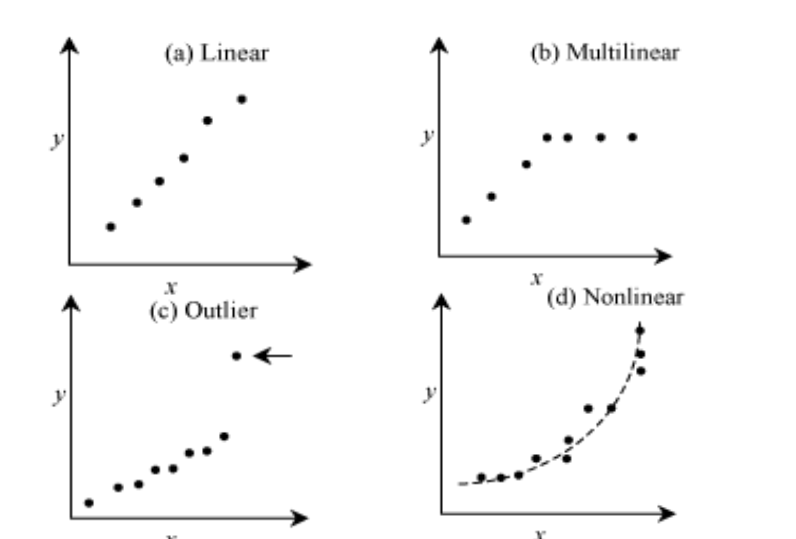
\includegraphics[width=.7\textwidth]{img/chapter-5/regression-relations.png}
\caption{Esempi di dati in relazione tra loro}\label{img:regression-relations}
\end{figure}

\subsubsection{Indipendenza degli errori}
Per verificare l'indipendenza degli errori a livello grafico, si va a plottare la distribuzione degli errori \(e_i\) rispetto alle corrispettive variabili predette \(\hat{y}_i\), ciò viene fatto per verificare se ci sia dipendenza in base alla variabile predetta, e quindi "scagionare" dei trend indesiderati all'interno degli errori. Per comprendere tale concetto, visualizzare l'immagine [\ref{img:independent-errors}], che mostra degli esempi di errori sia indipendenti, che dipendenti in diverse forme.

\begin{figure}[h]
\centering
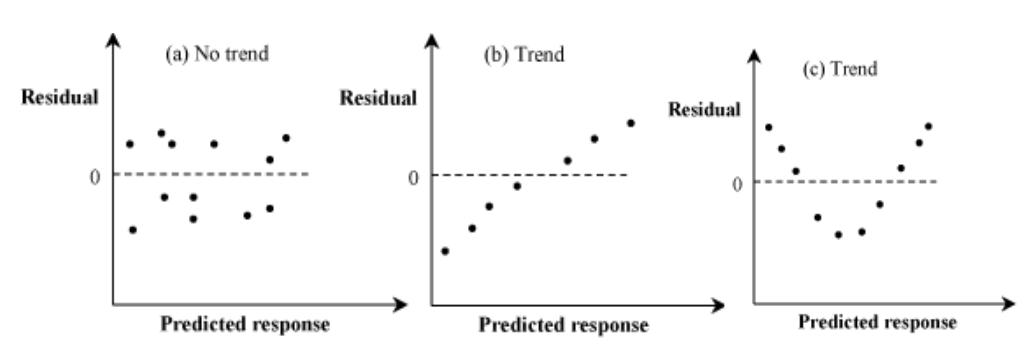
\includegraphics[width=.8\textwidth]{img/chapter-5/independet-errors.png}
\caption{Esempi di distribuzioni degli errori rispetto alla variabile \(\hat{y}_i\)}\label{img:independent-errors}
\end{figure}

A volte, è conveniente andare a plottare gli errori \(e_i\) in riferimento al numero dell'esperimento stesso \(i\), in modo da verificare se magari ci sono effetti nascosti (errata inizializzazione, procedure sperimentali) o delle condizioni dell'ambiente (temperatura ed umidità) che vanno ad incidere su tali errori (per fare ciò vado sempre a verificare i possibili trend presenti all'interno di tale relazione). Esempi di tali plot sono quelli presenti in figura [\ref{img:errors-side-effect}]

\begin{figure}[h]
\centering
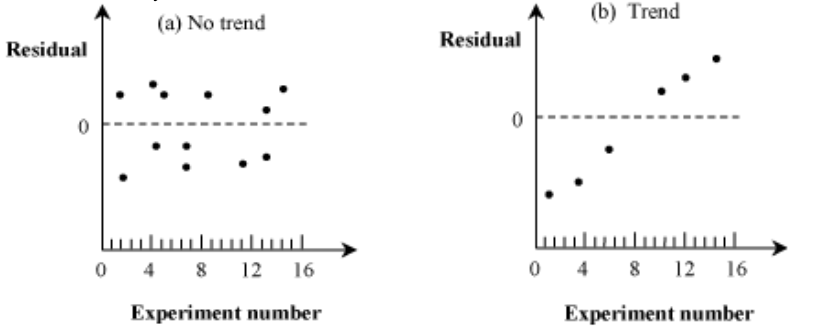
\includegraphics[width=.7\textwidth]{img/chapter-5/errors-side-effect.png}
\caption{Plotting degli errori rispetto alla posizione di valutazione}\label{img:errors-side-effect}
\end{figure}

\subsubsection{Errori distribuiti normalmente}
Per verificare se gli errori seguono una distribuzione normale, ci viene in aiuto il \textbf{Quantile-Quantile plotting}, che mette in relazione la distribuzione ottenuta dagli errori, rispetto ad una distribuzione normale. Esempi di applicazione della QQ-Plot sono rappresentati in figura [\ref{img:qqplot-errors}]

\begin{figure}[h]
\centering
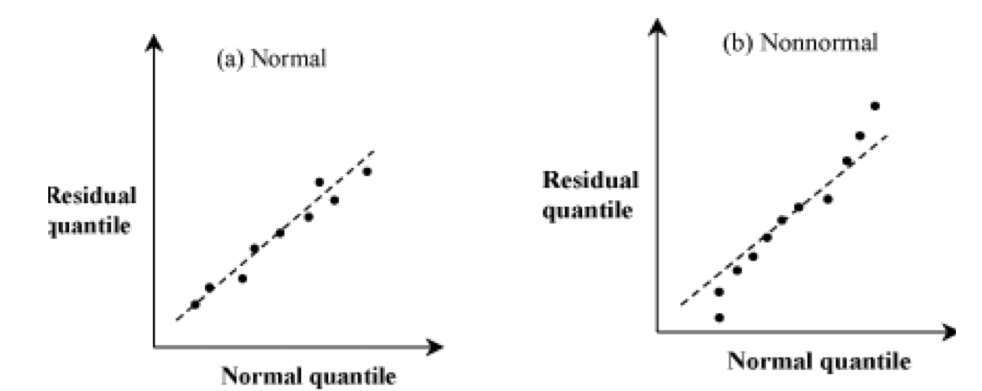
\includegraphics[width=.7\textwidth]{img/chapter-5/qqplot-errors.png}
\caption{QQ-Plot per le distribuzioni degli errori}\label{img:qqplot-errors}
\end{figure}

\subsubsection{Deviazione standard costante}
Quello che si va a fare, si va a plottare gli errori in riferimento alla risposta predetta (che dipende dalle predictor variables), andando a valutare se ci sono relazioni. Tale test visivo ci permette di verificare l'\textbf{Omoschedasticità}(Deviazione standard costante e media nulla) [Questa è la definizione mostrata a lezione e dalle dispense, anche se sui testi e in rete la definizione comprende solo la parte di deviazione standard (solo ipotesi di costanza di tale valore)]. Guardando il grafico, è importante stare attenti ad osservare se c'è un trend degli errori rispetto alla risposta predetta. Poichè in tal caso, non si possono fare ipotesi sulla costanza della varianza. Esempi di tali grafici sono quelli mostrati alla figure [\ref{img:constant-deviation}]

\begin{figure}[h]
\centering
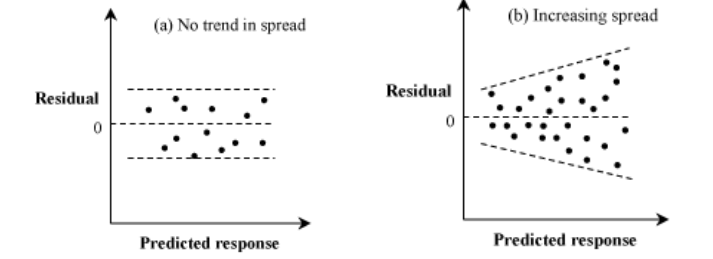
\includegraphics[width=.7\textwidth]{img/chapter-5/constant-deviation.png}
\caption{Distribuzione degli errori}\label{img:constant-deviation}
\end{figure}


L'Omoschedasticità si può verificare (o confermare) anche mediante l'utilizzo di uno specifico test statistico. Vi sono varie tecniche e modelli con cui tale test può essere effettuato, tali tecniche vanno sotto il nome di ANOVA (Analysis Of Variance) in letteratura. Ad esempio: 
\begin{itemize}

  \item \textbf{p-value:} 
  È la probabilità di osservare un risultato uguale o più estremo di quello ottenuto, assumendo vera l’ipotesi nulla. 
  Nei test di uguaglianza delle varianze indica quanto è plausibile che le varianze siano effettivamente uguali. 
  Se $p < \alpha$ (es. 0.05), si rifiuta l’ipotesi nulla: le varianze non sono uguali.

  \item \textbf{Test di Levene:} 
  Verifica se le varianze di più campioni sono uguali, basandosi sulle deviazioni assolute dalla media (o mediana) di ciascun campione. 
  È più robusto del test di Bartlett rispetto alla non-normalità. 
  Ipotesi nulla: le varianze dei campioni sono uguali.

  \item \textbf{Test di Brown–Forsythe:} 
  Variante del test di Levene che utilizza la mediana invece della media, rendendolo ancora più robusto a outlier e distribuzioni asimmetriche. 
  Ipotesi nulla: le varianze dei campioni sono uguali. 
  È consigliato quando la normalità non può essere assunta.

  \item \textbf{Test di Bartlett:} 
  Test classico per verificare l’uguaglianza delle varianze basato su una statistica $\chi^2$. 
  È potente se i dati sono normali, ma molto sensibile alle deviazioni dalla normalità. 
  Ipotesi nulla: tutte le varianze sono uguali; se $p < \alpha$, si conclude che almeno una varianza differisce.
    
  \item Ce ne sono altri ma prescindono da tale corso

\end{itemize}

Nel caso in cui, invece, i dati siano normali ma Eteroschedatici, allora è conveniente utilizzare il \textbf{Welch's t-test}. 

\begin{warn}
Le specifiche fatte sulle varie tecniche sopraelencate sono state aggiunte per un leggero grado di comprensione in più. Ma non sono richieste al fine di effettuare l'esame
\end{warn}

\subsection{Regressione Lineare Non parametrica}
Quando si parla di \textbf{Regressione lineare non parametrica}, si intende quell'insieme di tecniche che cerca un trend di un certo tipo, senza fare alcuna ipotesi sulla forma della popolazione o sulla distribuzione che i dati devono avere, richiede solo che ci sia indipendenza sui dati presenti. 
Per tali tipologie di test si utilizza il \textbf{test di Mann-Kendal}, che va a valutare la tendenza di una serie, e verifica se questa sia monotona o meno. Formalizzando tale concetto, andiamo a definirne le specifiche:
\\
Dato un insieme di una coppia di valori, di cui si vuole verificare un eventuale trend (insieme di punti nel piano), \(x_1, x_2, \dots, x_n\) e \(y_1, y_2, \dots, y_n\), si definisce un valore \(S\) che sarà utilizzato per la verifica. Sì definisce il valore \(S\) come:
\[
S = \sum_{i < j}sign((x_j - x_i)(y_j-y_i))
\]
Quindi si va ad effettuare una somma della valutazione dei parametri (se concordi si somma, se discordi si sottrae).
Più precisamente si va a controllare se i punti siano \textbf{concordanti} (Concordant, danno un contributo positivo) o \textbf{discordanti} (discordant, danno un contributo negativo). Per comprendere tale relazione guardare l'immagine [\ref{img:concordant-discordant}].

\begin{figure}[h]
\centering
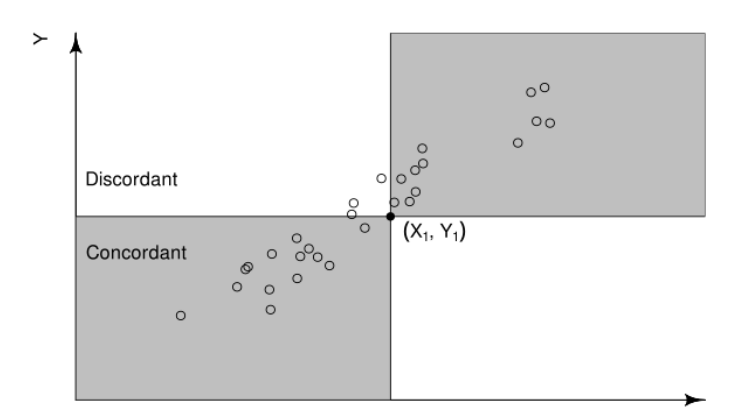
\includegraphics[width=.7\textwidth]{img/chapter-5/concordant-discordant.png}
\caption{Punti concordanti e discordanti}\label{img:concordant-discordant}
\end{figure}

Il valore di \(S\) ci permette di capire, in base al segno ed al valore che assume, se i dati hanno una certa tendenza. Per capire al meglio tale tendenza, ci calcola un'altro parametro \(\tau_a\) che indica il \textbf{coefficente di correlazione}. Più \(S\) e \(\tau_a\) sono grandi e più con forza posso rigettare l'ipotesi nulla (quella associata alla mancanza di trend nei dati). 
Per calcolare la \(\tau_a\) si effettua il seguente calcolo
\[
\tau_a = \frac{S}{\binom{n}{2}} = \frac{S}{\frac{n(n-1)}{2}}
\]
Con tale valore, vado a riscalare il valore di \(S\) ad un range \(-1 \leq \tau_a \leq 1\), poichè è come se stessi andando ad aggiungere un peso per ogni valore "valutato".

Dato che solitamente, si potrebbe incappare nel problema dei "pareggi" (ovvero valori nulli). Si può andare a valutare un'altro parametro che è:
\[
\tau_b = \frac{S}{\sqrt{(\binom{n}{2} - n_1)(\binom{n}{2}-n_2)}}
\]
Dove \(n_1\) ed \(n_2\) sono il numero di pareggi per ogni campione che si va a considerare (\(x_i\) ed \(y_i\)).

\subsubsection{Procedura di Sen}
Un modo per essere più robusti agli outlier e trovare un eventuale trend, è la seguente procedura. Considerato che i dati mostrati \textbf{posseggono tra loro un trend}, si vanno a valutare le pendenze, e si seleziona il valore della mediana tra queste.
Per la valutazione delle pendenze si prosegue nel seguente calcolo:
\[
slope_{ij} = \frac{y_j - y_i}{x_j - x_i}
\]

\section{Altri modelli di regressione}
A volte la \textbf{Simple linear regression} non riesce a compensare tutti i casi richiesti o leggermente più complessi. Pertanto è utile andare ad esplorare diverse tecniche che ne permettono una buona stima

\subsection{Regressione Lineare Multipla}
A differenza della regressione lineare semplice, dove si cerca una relazione tra una singola variabile predictor e una singola predictable variable. Talvolta, utilizzare tale metodologia può essere limitante. Pertanto si definisce la \textbf{Multiple Linear Regression}(Regressione Lineare Multipla), che va a considerare una relazione \textbf{lineare} tra diverse variabili predictor. Per ogni campione si effettua una predizione rispetto al numero di parametri che si sono andari a utilizzare (predictor variables). Formalmente, definendo:
\begin{itemize}
    \item \(\mathbf{x_{ij}}\): Valore dell'attributo j-esimo per il campione i-esimo
    \item \(\mathbf{y_j}\): j-esimo valore predetto
    \item \(\mathbf{b_i}\): coefficente associato al parametro i-esimo
    \item \(\mathbf{e_j}\): Errore associato al j-esimo valore predetto
\end{itemize}

si può scrivere la relazione tra i predictor variables e le predictable variables come:
\[
y_j = b_0 + b_1 x_{j1} + b_2 x_{j2} + \dots + b_k x_{jk} + e_j
\]
Oppure in maniera estesa come:
\[
\begin{bmatrix}
y_1 \\
y_2 \\
\dots\\
y_n
\end{bmatrix}
= 
\begin{bmatrix}
1 & x_{11} & x_{12} & \dots & x_{1k}\\
1 & x_{21} & x_{22} & \dots & x_{2k}\\
\dots & \dots & \dots & \dots & \dots \\
1 & x_{n1} & x_{n2} & \dots & x_{nk}
\end{bmatrix}
\begin{bmatrix}
b_0 \\
b_1 \\
\dots \\
b_n
\end{bmatrix}
+
\begin{bmatrix}
e_1\\
e_2\\
\dots\\
e_n
\end{bmatrix}
\]
Con la notazione vettoriale
\[
\mathbf{\underline{y}} = \underline{\underline{\mathbf{X}}}\ \underline{\mathbf{b}}+\underline{\mathbf{e}}
\]

Per il calcolo dei parametri, si cerca di andare a minimizzare la formula dell'errore, ovvero:
\[
e_i = y_i - b_0 - b_1 x_{i1} - b_2 x_{i2} - \dots - b_k x_{ik} 
\]
\[
\sum_{i=1}^{n}e_i^2 = \sum_{i=1}^{n}(y_i - b_0 - b_1 x_{i1} - b_2 x_{i2} - \dots - b_k x_{ik})^2
\]

Scrivendo \(\sum_{i=1}^{n}e_i^2 = (\underline{y}-\underline{\underline{X}}\ \underline{b})^T(\underline{y}-\underline{\underline{X}} \ \underline{b})\), da cui, derivando rispetto a \(b\), si ottiene:
\[
\underline{b} = (\underline{\underline{X}}^t\ \underline{\underline{X}})^{-1}\underline{\underline{X}}^T\ \underline{y}
\]

Compreso come effettuare la stima dei valori per effettuare la regressione lineare multipla, si prosegue nell'effettuazione della valutazione degli "errori", delle veriazioni e delle devianze.
Precisamente, partendo dalle variazione e dalle devianze, si ha che:
\[
SSY = \sum_{i=1}^{n}y_i^2, SS0= n\overline{y}^2
\]
\[
SST = SSY - SS0
\]
\[
SSR = SST - SSE
\]

Dove i gradi di libertà della SST sono sempre \(n-1\) mentre quelli della SSE sono \(n-k-1\). Si valutano, anche, il coefficiente di determinazione e la deviazione standard, come:
\[
R^2 = \frac{SSR}{SST}
\]
\[
s_e = \sqrt{\frac{SSE}{n-k-1}}
\]

Per il calcolo del \textbf{MSE}(Mean squared error), si effettua la seguente formula:
\[
MSE = \frac{SSE}{n-k-1}
\]

Mentre la deviazione standard dei parametri, viene valutata come:
\[
s_{b_j} = s_e\sqrt{c_{jj}} 
\]

dove \(c_{jj}\) è il j-esimo elemento diagonale della matrice \(\underline{\underline{C}} = (\underline{\underline{X}}^T\underline{\underline{X}})^{-1}\)

\subsection{Multicolinearità}
La \textbf{Multicolinearità} vuol dire effettuare la regressione con una dipendenza lineare tra le variabili predictor (tale situazione è detta colineare). Tale situazione, ci permette di capire che si avrebbe una variabile in più su cui si sta effettuando la regressione (quindi di per se, inutile). Quindi, solitamente, è utile capire se due variabili sono colineari o meno (correlate o meno). Per effettuare tale valutazione si va a calcolare la correlazione tra i due elementi, che poi viene valutata.
La correlazione tra i due elementi viene calcolata come:
\[
Correlation(x_1,x_2) = R_{x_1x_2} = 
\]
\[
=\frac{\sum_{i=1}^{n}x_{1i}x_{2i} - \frac{1}{n}\left(\sum_{i=1}^{n}x_{1i}\right)\left(\sum_{i=1}^{n}x_{2i}\right)}{\left[\sum_{i=1}^{n}x_{1i}^2 - \frac{1}{n}\left(\sum_{i=1}^{n}x_{1i}\right)\left(\sum_{i=1}^{n}x_{1i}\right) \right]^{1/2}\left[\sum_{i=1}^{n}x_{2i}^2 - \frac{1}{n}\left(\sum_{i=1}^{n}x_{2i}\right)\left(\sum_{i=1}^{n}x_{2i}\right) \right]^{1/2}}
\]

Quindi, aggiungere una variabile predictor non è detto che sia sempre una buona idea, poichè, la correlazione tra due predittori, riduce l'accuracy e va ad amplificare la varianza (Valori della matrice di correlazione vista in precedenza). 

\subsection{Regressione Curvilinea}
Talvolta, può capitare che la relazione presente tra \(y\) e \(x\) non sia lineare, ma che comunque racchiude una funzione non lineare. Quello che sostanzialmente si può andare a fare, è cercare una relazione lineare rispetto a funzioni non lineari. Per capire, immaginiamo che \(y\) ed \(x\) siano legate dalla legge \(y = bx^\alpha\), allore quello che si potrebbe andare a fare, è valutare il modello logaritmico di tale funzione come:
\[
ln(y) = ln(b)+ \alpha ln(x)
\]

Il che quindi mi consente di utilizzare le tecniche affrontate per la regressione lineare, per trovare i valori di \(b\) e \(\alpha\). Oltre a tale legame ce ne sono altri, che sono mostrati nella figura [\ref{img:trasformazioni-curvilinee}]

\begin{figure}[h]
\centering
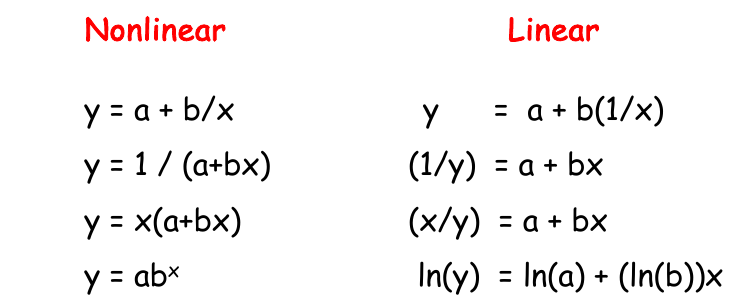
\includegraphics[width=.7\textwidth]{img/chapter-5/relazioni-curvilinee.png}
\caption{Forme di trasformazione di funzioni non lineari in relazioni lineari}\label{img:trasformazioni-curvilinee}
\end{figure}

\subsection{Outliers}
